%%%%%%%%%%%%%%%%%%%%%%%%%%%%%%%%%%%%%%%%%%%%%%%
%%% Template for lab reports used at STIMA
%%%%%%%%%%%%%%%%%%%%%%%%%%%%%%%%%%%%%%%%%%%%%%%

%%%%%%%%%%%%%%%%%%%%%%%%%%%%%% Sets the document class for the document
% Openany is added to remove the book style of starting every new chapter on an odd page (not needed for reports)
\documentclass[11pt,polish, openany]{book}

%%%%%%%%%%%%%%%%%%%%%%%%%%%%%% Loading packages that alter the style
\usepackage[]{graphicx}
\usepackage[]{color}
\usepackage{alltt}
\usepackage[T1]{fontenc}
\usepackage[utf8]{inputenc}
\setcounter{secnumdepth}{3}
\setcounter{tocdepth}{3}
\setlength{\parskip}{\smallskipamount}
\setlength{\parindent}{0pt}

% Set page margins
\usepackage[top=100pt,bottom=100pt,left=68pt,right=66pt]{geometry}

% Package used for placeholder text
\usepackage{lipsum}

% Prevents LaTeX from filling out a page to the bottom
\raggedbottom

% Adding both languages
\usepackage[english, polish]{babel}

% All page numbers positioned at the bottom of the page
\usepackage{fancyhdr}
\fancyhf{} % clear all header and footers
\fancyfoot[C]{\thepage}
\renewcommand{\headrulewidth}{0pt} % remove the header rule
\pagestyle{fancy}

% Changes the style of chapter headings
\usepackage{titlesec}
\titleformat{\chapter}
   {\normalfont\LARGE\bfseries}{\thechapter.}{1em}{}
% Change distance between chapter header and text
\titlespacing{\chapter}{0pt}{50pt}{2\baselineskip}

% Adds table captions above the table per default
\usepackage{float}
\floatstyle{plaintop}
\restylefloat{table}

% Adds space between caption and table
\usepackage[tableposition=top]{caption}

% Adds hyperlinks to references and ToC
\usepackage{hyperref}
\hypersetup{hidelinks,linkcolor = black} % Changes the link color to black and hides the hideous red border that usually is created

% If multiple images are to be added, a folder (path) with all the images can be added here 
\graphicspath{ {Figures/} }

% Separates the first part of the report/thesis in Roman numerals
\frontmatter

%%%%%%%%%%%%%%%%%%%%%%%%%%%%%% Starts the document
\begin{document}

%%% Selects the language to be used for the first couple of pages
\selectlanguage{polish}

%%%%% Adds the title page
\begin{titlepage}
	\clearpage\thispagestyle{empty}
	\centering
	\vspace{1cm}

	% Titles
	% Information about the University
	{\normalsize Uniwersytet Technologiczno-Przyrodniczy \\ 
		im. Jana i Jędrzeja Śniadeckich \\
		w Bydgoszczy \par}
		\vspace{3cm}
	{\Huge \textbf{Projektowanie i programowanie gier}} \\
	%\vspace{1cm}
	%{\large \textbf{xxxxx} \par}
	\vspace{4cm}
	{\normalsize DOKUMENTACJA PROJEKTU GRY GOTHIC \\ % \\ specifies a new line
	             Paweł Rudnicki 110974 \\
	             Norbert Skulski 110797\par}
	\vspace{5cm}
    
    \centering 
\includegraphics[scale=0.5]{utp.png}
    
    \vspace{0.5cm}
		
	% Set the date
	{\normalsize 12-03-2020 \par}
	
	\pagebreak

\end{titlepage}

% Adds a table of contents
\tableofcontents{}

%%%%%%%%%%%%%%%%%%%%%%%%%%%%%%%%%%%%%%%%%%%%%%%%%%%%%%%%%%%%%%%%%%%%%%%%%%%%%%%%%%%%%%%%%%%%
%%%%%%%%%%%%%%%%%%%%%%%%%%%%%%%%%%%%%%%%%%%%%%%%%%%%%%%%%%%%%%%%%%%%%%%%%%%%%%%%%%%%%%%%%%%%
%%%%% Text body starts here!
\mainmatter

\chapter{Wstępny abstrakt}\label{chapt:sum}
Fabuła gry opowiada historię o bezimiennym bohaterze w kolonii karnej znanej również jako Górnicza Dolina.
Jest ona usytuwana na wyspie Khorinis, która została otoczona magiczną barierą, którą można pokonać
tylko ze strony świata zewnętrznego ponieważ wszelkie próby wydostania się z jej wnętrza kończą się tragicznie.
Magiczna bariera została stworzona przez magów na rozkaz króla Rhobara II w celu zapobiegnięcia kradzieży
magicznej rudy wydobywanej w owej dolinie, którą potrzebował do produkcji broni.
Król Rhobar II pokonał niemal wszystkich wrogów swojego królestwa. Poza orkami. Trzeba rzec, że nigdy nie grzeszyli
inteligencją, lecz ich główną umiejętnością jest formowanie szyków przejawiających się przeogromną siłą, i 
determinacją, które są nieodzowną zaletą w celu osiągnięcia końca gatunku ludzkiego. Historia gry rozpoczyna się, kiedy
główny bohater trafia do Górniczej Doliny jako kolejny, nic nie znaczący jeniec, którym został poprzez narażenie się na drobne
kradzieże wbrew interesu królestwa. Zanim zostanie on zesłany, i przejdzie przez magiczną barierę otrzymuje list od Maga Ognia
zaadresowany do Najwyższego Maga Ognia stacjonującego w tak zwanym Starym Obozie, który jest jednym z trzech głównych obozów rozśanych po
Górniczej Dolinie. Defakto, nie jest to jego jedyny cel jaki otrzymał. Bezimienny bohater chce również uciec z Górniczej Doliny, jak tylko będzie
potrafił.

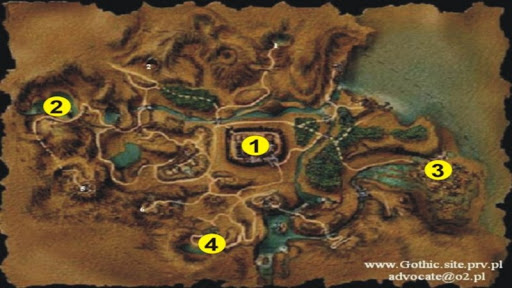
\includegraphics[scale=0.9]{mapa.jpg}

Świat jaki gracz ma do dyspozycji to już wspomniana wcześniej Górnicza Dolina, w której znajdują się trzy obozy konkurujące ze sobą o wszelakie zasoby pozwalające przetrwać w tym brutalnym świecie oraz wieża tajemniczego maga Xardasa.
\begin{itemize}
    \item [1] \textbf{Stary Obóz} - Najstarszy ze wszystkich obozów, mieszczący się na terenie zamku, w którym niegdyś mieszkała straż królewska, magnaci, magowie ognia oraz kopacze, a który po stworzeniu bariery został przejęty przez więźniów. W odróżnieniu od reszty ten obóz rządzi się surowymi prawami. Posiada kopalnię magicznej rudy. Tylko ten obóz prowadzi wymianę z królem, chociaż Nowy Obóz także posiada swoją kopalnię. Z trzech obozów tylko ten nie planuje zniszczyć bariery, jego celem jest wyłącznie handel z królem i Obozem Bractwa. Dzięki temu jest najbogatszy ze wszystkich. Rhobar II, w zamian za magiczną rudę, oddaje wszystko, czego Stary Obóz zażąda. Stary Obóz otoczony jest drewnianą palisadą i dzieli się na zewnętrzny pierścień, w którym żyją kopacze i cienie, oraz wewnętrzny (zamek), gdzie przebywają strażnicy, magowie ognia i magnaci. Przywódcą Starego Obozu jest magnat o imieniu Gomez. W zewnętrznym pierścieniu znajduje się również arena, gdzie walczą przedstawiciele trzech obozów, a także plac targowy. Inne grupy więźniów również posiadają swoich przywódców. Przywódcą strażników jest Thorus, cieni – Diego, a magów ognia – Corristo.
    \item [2] \textbf{Nowy Obóz} - Obóz powstały jako efekt rozłamu w Starym Obozie. Dąży do zniszczenia magicznej bariery i uwolnienia więźniów poprzez detonację wielkiego kopca rudy. Potrzebny w tym celu surowiec wydobywają w Wolnej Kopalni krety. Większość domostw, siedziba magów wody oraz góra rudy znajduje się w wielkiej jaskini. Członkowie Nowego Obozu to głównie dezerterzy i uciekinierzy ze Starego Obozu. W tym obozie nie ma zasad, a prawo to tylko abstrakcyjne pojęcie. By jednak chronić wielki kopiec magicznej rudy, magowie wody zatrudnili najemników, którzy chronią ich i kopiec przed szkodnikami. Jest to, mimo ogromnej ilości posiadanej rudy, najbiedniejszy obóz, utrzymujący się głównie z napadów na konwoje Starego Obozu, przez co znajdują się o krok od wojny domowej. Dzięki tamie wodnej i odpowiednim warunkom możliwa jest uprawa ryżu, który służy m.in. do produkcji ryżówki – alkoholu sprzedawanego w karczmie. Przywódcą najemników w Nowym Obozie jest Generał Lee, wtrącony do kolonii za morderstwo, którego nie popełnił. Przywódcą szkodników jest Lares, a arcymistrzem magów wody – Saturas.
    \item [3] \textbf{Obóz Bractwa} - Jest to obóz (nazywany również Obozem na Bagnie lub Obozem Sekty), którego członkowie wyrzekli się starych bogów, czcząc Śniącego, który ma im pomóc w odzyskaniu wolności. Dzięki wizji Y'Beriona, duchowego przywódcy bractwa, uwierzyli, że Śniący ma za zadanie pomóc wiernym, niszcząc barierę, a niewiernych ukarać. Obóz Sekty propaguje palenie bagiennego ziela, rosnącego tylko tutaj. Każdy nowicjusz dostaje dzienną porcję, by móc pozostać w duchowym kontakcie ze Śniącym. Niektórzy guru po większej ilości bagiennego ziela mają wizje dotyczące Śniącego. Przez pozostałych więźniów członkowie bractwa są uważani za świrów, czy też wariatów, być może z powodu tatuaży na ciele, dziwnych strojów, całkowicie ogolonych głów lub po prostu odmiennych wierzeń. Wielu więźniów dołącza do tego obozu głównie z powodu bagiennego ziela i jego specjalnych właściwości. Obóz składa się z drewnianych domów stojących na ziemi i zawieszonych na drzewach oraz świątyni, w której mieszka Y'Berion wraz z Natalią i Chani, które najprawdopodobniej są jego kurtyzanami. Mieszkańcy obozu dzielą się na nowicjuszy, których głównym zadaniem jest zbieranie i obróbka bagiennego ziela, guru, którzy otrzymują wizje od Śniącego oraz strażników świątynnych, którzy pilnują bezpieczeństwa, a także zbierają wydzielinę pełzaczy – potworów podobnych do wielkich pająków nękających kopaczy w Starej Kopalni. Ośmiu guru przewodzi obozowi. Najwyższy z nich to Y'Berion, którego zastępcą jest Cor Kalom, a trzecią najważniejszą osobą w całym bractwie jest Cor Angar. Pozostałych pięciu guru to Baal Namib, Baal Cadar, Baal Tyon, Baal Orun i Baal Tondral.
    \item [4] \textbf{Wieża Xardasa} - druga wieża nekromanty Xardasa. Znajduje się w samym środku terytoriów należących do orków, w małej kotlince niedaleko miasta orków. Jest także najbardziej wysuniętym na południe punktem Górniczej Doliny.Xardas wzniósł ją po zniszczeniu poprzedniej wieży z pomocą służących mu ożywieńców. Droga do wieży jest bardzo ciężka i pełna niebezpieczeństw. Dostać się do niej można idąc przez wąski wąwóz, który broniony jest przez kamiennego golema, lodowego golema oraz ognistego golema
\end{itemize}
\chapter{Rozszerzone streszczenie gry}
Akcja gry rozgrywa się na terenie kopalni Korinis osadzonej w Górniczej dolinie.
Ówczesny król Myrtany Robar II toczący wojnę z orkami potrzebował surowców aby dostarczyć swoim wojską wyposażenie. Nakazał więc wysłanie wszystkich skazańców z królestwa do Korinis aby przeprowadzali wydobycie potrzebnych zasobów. By uniemożliwić im ucieczkę nakazał stworzenie magicznej bariery.
Podczas tworzenia magicznej bariery nie wszystko poszło zgodnie z planem i uwięziła ona również magów ja tworzących.
\newline
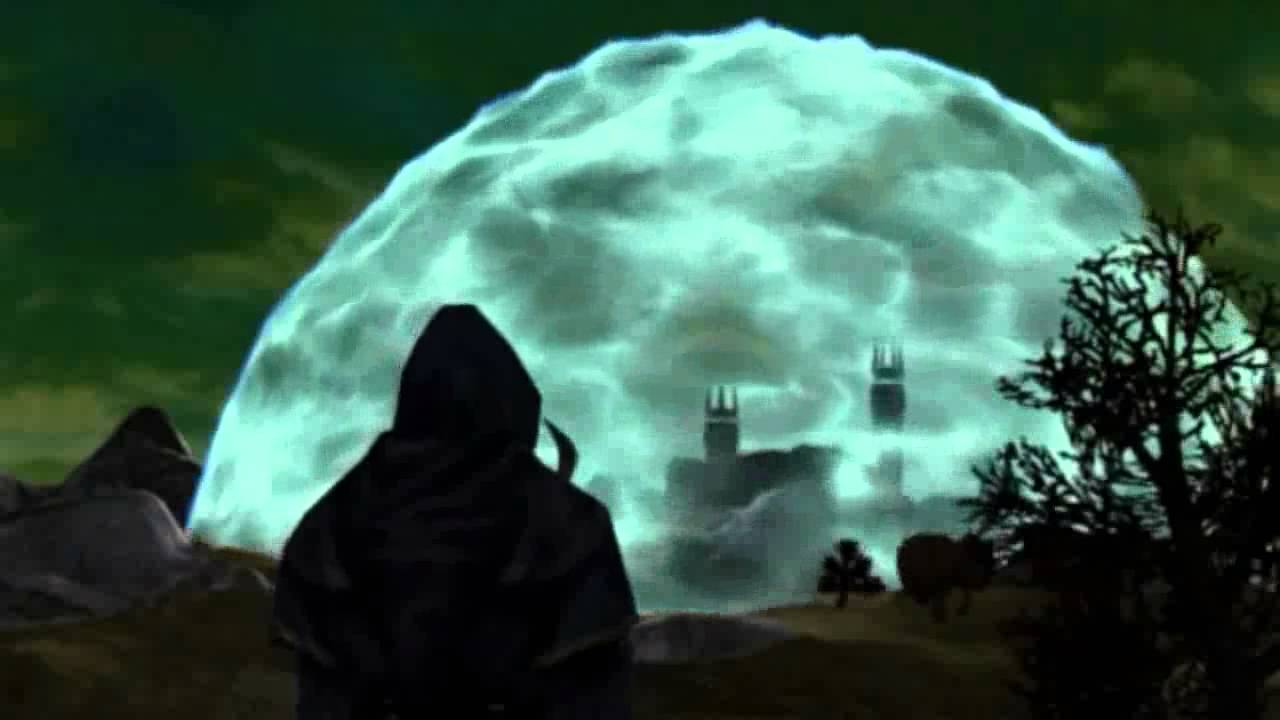
\includegraphics[scale=0.37]{bariera}
\newline
Bohater gry to więzień o nieznanym imieniu, Zostaje wtrącony do kolonii karnej za nieznane graczowi przestępstwo.  Przed wtrąceniem dostaje od maga zadanie dostarczenia listu do jego pobratymców znajdujących się pod drugiej stronie bariery. Po wtrąceniu na teren bariery przechodzi „Chrzest”. Zostaje pobity przez znajdujących się tam więźniów. Przed śmiercią ratuje go wysoko postawiony łucznik ze starego obozu o imieniu Diego. Od tamtej pory jednym z jego początkowych zadań jest staranie się o przynależność do jednego z obozów. W tym celu Bezimienny musi wykonywać zadania zlecane mu przez ważne osobistości w wybranym obozie.
Po przystąpieniu do którejkolwiek frakcji bohater otrzymuje od jej władz polecenie pomocy Bractwu Śniącego w przygotowaniach rytuału nawiązania kontaktu z Śniącym. Wyznawcy Śniącego wierzą, że gdy dojdzie do przebudzenia ich śpiącego boga, pomoże im on wydostać się z kolonii karnej. Skazaniec otrzymuje prawo do audiencji u przywódcy Bractwa – Y'Beriona. Każe on odnaleźć bohaterowi kamień ogniskujący – artefakt, który był wykorzystywany w procesie tworzenia magicznej bariery.
\newline
\begin{center}
	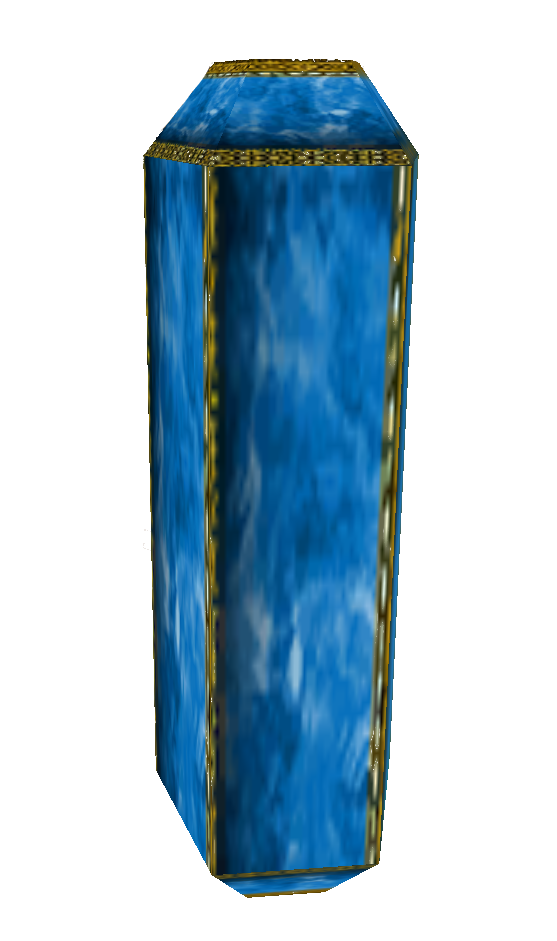
\includegraphics[scale=0.2]{kognisk}
\end{center}

Po odnalezieniu kamienia alchemik Bractwa imieniem Cor Kalom informuje Bezimiennego, że do przygotowania rytuału potrzebna jest mu wydzielina żyjących w Starej Kopalni groźnych stworzeń zwanych pełzaczami. W tym celu Bractwo regularnie wysyła do kopalni strażników świątynnch, którzy przynoszą Cor Kalomowi wnętrzności zabitych stworzeń. Cor Kalom uważa jednak, że musi istnieć efektywniejsze źródło wydzieliny niż wnętrzności pełzaczy i wysyła bohatera na wyprawę celem znalezienia go. Bohater udaje się do kopalni, gdzie odkrywa lokalizację gniazda stworzeń. Dostaje się do niego, pokonuje ich królową i zabiera jaja pełzaczy do Cor Kaloma. Ostatnią rzeczą potrzebną do przeprowadzenia rytuału jest księga zwana Almanachem – zawiera ona instrukcje wykorzystywania kamienia ogniskującego. Bezimienny znajduje ją w jaskini będącą kryjówką wrogo nastawionych czarnych goblinów.
Uczestnikom rytuału objawia się wizja ruin, w których rezydują orkowie. Tuż po zakończeniu wizji przewodzący ceremonii Y'Berion traci przytomność. Bezimienny zostaje wysłany na pomoc ekspedycji wysłanej w celu zbadania leżącego w pobliżu obozu Bractwa cmentarzyska orków. Na miejscu okazuje się, że ekspedycja zawiodła, a cmentarzysko nie zawiera żadnej wskazówki co do dalszych działań. Bohater wraca do obozu. Wkrótce potem Y'Berion umiera. Tuż przed śmiercią ostrzega przed dalszymi próbami budzenia Śniącego i upatruje nadziei na wolność w planie magów wody z Nowego Obozu. Plan ów polega na detonacji wielkiego kopca magicznej rudy. Na polecenie arcymaga wody imieniem Saturas Bezimienny odnajduje pozostałe kamienie ogniskujące i zostaje wysłany z misją przekonania magów ognia ze Starego Obozu do podjęcia próby zniszczenia bariery.
W międzyczasie dochodzi do podmycia Starej Kopalni przez podziemny zbiornik wodny. Kopalnia ta była źródłem przychodów dla Starego Obozu. Przywódca rządzących obozem magnatów imieniem Gomez rozkazuje przejąć zbrojnie należącą do Nowego Obozu Wolną Kopalnię. Mieszkający w Starym Obozie magowie ognia sprzeciwili się planom władz obozu i zostali wymordowani z rozkazu magnatów. Aby uniknąć odwetu ze strony Nowego Obozu, Gomez nakazuje strażnikom zamknięcie bram oraz atakowanie każdego, kto się do nich zbliża. Jeśli Bezimienny podjął decyzję o zostaniu członkiem Starego Obozu to zostanie z niego usunięty. W wyniku braku możliwości skorzystania z pomocy magów ognia Saturas informuje bohatera o trzynastym magu uczestniczącym w procesie tworzenia bariery o imieniu Xardas i każe go odnaleźć.
\newline
\begin{center}
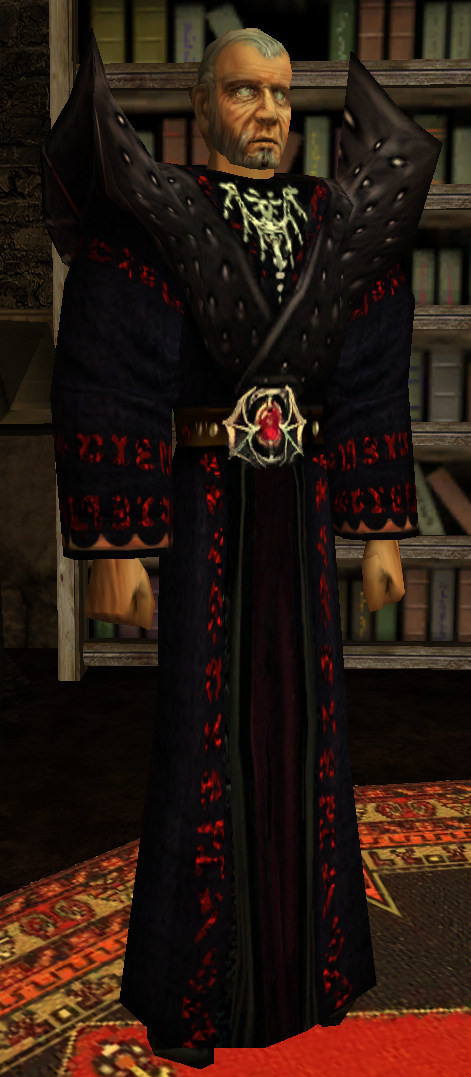
\includegraphics[scale=0.5]{xardas}
\end{center}

Xardas to nekromanta, który mieszka samotnie w wieży na środku terytorium zajętego przez orków. Po odnalezieniu go bohater dowiaduje się, że ma on własny pomysł na zniszczenie bariery i że plan magów wody jest nieskuteczny. Zleca on Bezimiennemu odnalezienie zbuntowanego orkowego szamana imieniem Ur-Shak, ochronienie go przed tropiącymi go pobratymcami oraz przesłuchanie go. Ur-Shak informuje nas, że Śniący jest demonem przywołanym przed wiekami przez orkowych szamanów z innego wymiaru. Sam zaś Śniący przebywa na dnie skomplikowanego podziemnego kompleksu jaskiń i korytarzy zwanym Świątynią Śniącego.
\newpage Wejście do świątyni znajduje się w Mieście Orków znajdującym się na terytorium tej rasy. Aby bezpiecznie poruszać się po terytorium orków i dotrzeć do ich miasta bohater potrzebuje amuletu o nazwie Ulu-Mulu. 
\newline
\begin{center}
	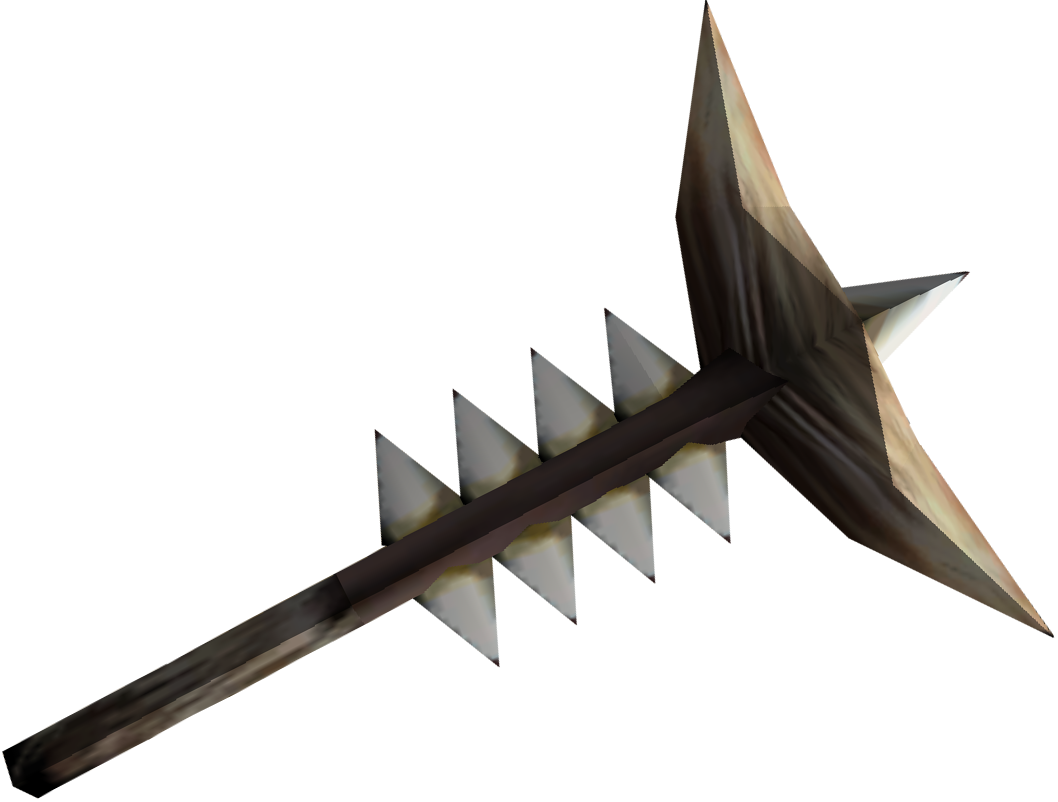
\includegraphics[scale=0.2]{umumulu}
\end{center}
Pomóc w jego wykonaniu ma Bezimiennemu przyjaciel Ur-Shaka pochwycony przez ludzi jako niewolnik i zmuszony do pracy w Wolnej Kopalni. Zdaniem Xardasa magia Śniącego wpłynęła na proces powstawania bariery i jedynym sposobem na zniszczenie jej jest wygnanie demona. Następnie, bohater wraz z najemnikiem Gornem z Nowego Obozu ruszają na odsiecz Wolnej Kopalni i odzyskują ją z rąk strażników Gomeza. Orkowy niewolnik pomaga Bezimiennemu wykonać amulet.
Po dotarciu do Miasta Orków bohater odnajduje wejście do Świątyni Śniącego i dostaje się do środka. Po drodze pokonuje orkowych szamanów-ożywieńców i zbiera ich oręż, który służy jako klucze do bram broniących dostępu do Śniącego. Ponadto Bezimienny odkrywa dodatkowy starożytny miecz o nazwie Uriziel pilnowany przez jednego z szamanów. Ten jednak jest bezużyteczny. Ostatni napotkany szaman okazuje się niewrażliwy na jakąkolwiek broń lub zaklęcie. Bohater wydostaje się ze świątyni i wraca do wieży Xardasa. Nekromanta opowiada mu historię znalezionego miecza. Zgodnie z sugestią nekromanty bohater wraz z jedynym ocalałym z rzezi magiem ognia wykorzystują kopiec magicznej rudy zgromadzony w Nowym Obozie do naprawy oręża. Bezimienny ściąga na siebie w ten sposób gniew magów wody.
Po ucieczce z Nowego Obozu bohater wraca do Świątyni Śniącego, pokonuje ostatniego szamana i dociera do leża demona. Na miejscu staje naprzeciw obudzonego Śniącego. Używając mieczy orkowych szamanów Bezimienny otwiera portal prowadzący do wymiaru, z którego przybył Śniący. Gra kończy się po tym, jak za pomocą Uriziela Bezimienny wtrąca przeciwnika do innego świata.

\chapter{Projektowanie świata gry}\label{chapt:doe}
Świat gry w którym rozgrywa się pierwsza część gry Gothic nastawiony jest przede wszystkim na takie cechy które ma odczuć gracz jak tajemniczość oraz mrok. Sama nazwa świata pozostaje nieznana, a tylko jego poszczególne lokacje.
\section{Górnicza Dolina}
\begin{center}
 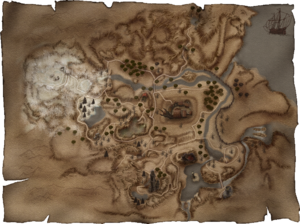
\includegraphics[scale=1.0]{dolina.jpg}
\end{center}
Górnicza Dolina jest połączona z morzem i znajduje się na południu wyspy Khorinis. Znajduje się tam wiele rodzajów krajobrazów: bagna, góry, pustkowia, lasy, plaże. Przepływają przez nią dwie rzeki. Pierwsza ma swoje źródło w górach na zachodzie za Nowym Obozem i dzieli się na dwie odnogi – jedną wpadającą prosto do morza oraz drugą, która spływa przez wodospady do bagien. Druga rzeka ma początek w jeziorku dookoła pierwszej wieży Xardasa. Z uwagi na klimat, który panuje na wyspie, roślinność występuje w wielu gatunkach i jest bardzo bujna. Teren porastają liczne, gęste lasy i puszcze. Żyje w niej zarówno wiele zwierząt łownych, jak i krwiożerczych bestii. Przestrzeń między obozami jest bardzo niebezpieczna, lecz po ścieżkach można stosunkowo łatwo i bezpiecznie podróżować. Górnicza Dolina dzieli się także na terytoria orków i ludzi. Znajdują się tam również trzy kopalnie rudy – dwie czynne i jedna zawalona. Na północy znajduje się przełęcz prowadząca do Khorinis, lecz niemożliwa do przebycia z powodu magicznej bariery. Stary Obóz znajduje się w samym środku kolonii. Na zachodzie, w górach znajduje się nowy obóz, na wschodzie zaś, na bagnach znajduje się obóz bractwa. Na południu znajdują się tereny orków. Są to niebezpieczne pustkowia pełne niebezpiecznych stworzeń jak ogniste jaszczury, brzytwy czy cieniostwory. Znajduje się tam miasto orków i wieża Xardasa.
\section{Stary obóz}
\begin{center}
 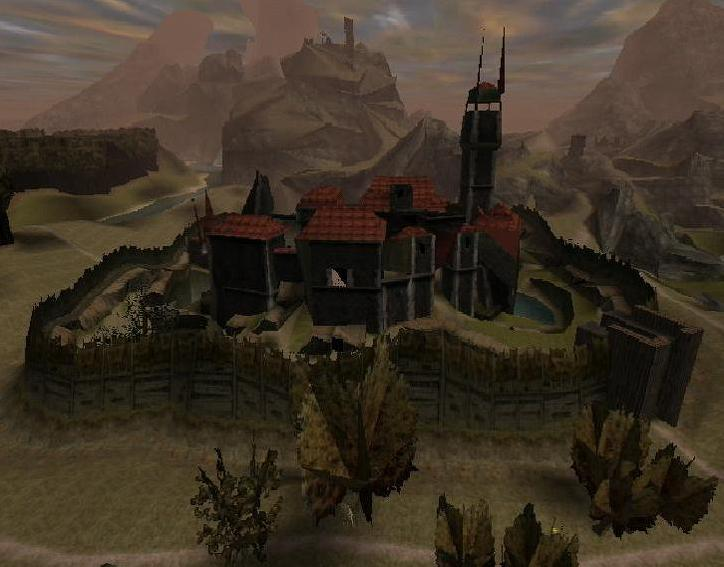
\includegraphics[scale=0.6]{staryoboz.jpg}
\end{center}
Najstarszy ze wszystkich obozów, mieszczący się na terenie zamku, w którym niegdyś mieszkała straż królewska, magnaci, magowie ognia oraz kopacze, a który po stworzeniu bariery został przejęty przez więźniów. W odróżnieniu od reszty ten obóz rządzi się surowymi prawami. Posiada kopalnię magicznej rudy. Tylko ten obóz prowadzi wymianę z królem, chociaż Nowy Obóz także posiada swoją kopalnię. Z trzech obozów tylko ten nie planuje zniszczyć bariery, jego celem jest wyłącznie handel z królem i Obozem Bractwa. Dzięki temu jest najbogatszy ze wszystkich. Rhobar II, w zamian za magiczną rudę, oddaje wszystko, czego Stary Obóz zażąda. Stary Obóz otoczony jest drewnianą palisadą i dzieli się na zewnętrzny pierścień, w którym żyją kopacze i cienie, oraz wewnętrzny (zamek), gdzie przebywają strażnicy, magowie ognia i magnaci. Przywódcą Starego Obozu jest magnat o imieniu Gomez. W zewnętrznym pierścieniu znajduje się również arena, gdzie walczą przedstawiciele trzech obozów, a także plac targowy. Inne grupy więźniów również posiadają swoich przywódców. Przywódcą strażników jest Thorus, cieni – Diego, a magów ognia – Corristo. Udzwiękowienie danej lokacji powinno budzić u gracza poczucie bezpieczeństwa i spokoju.
\section{Nowy obóz}
\begin{center}
 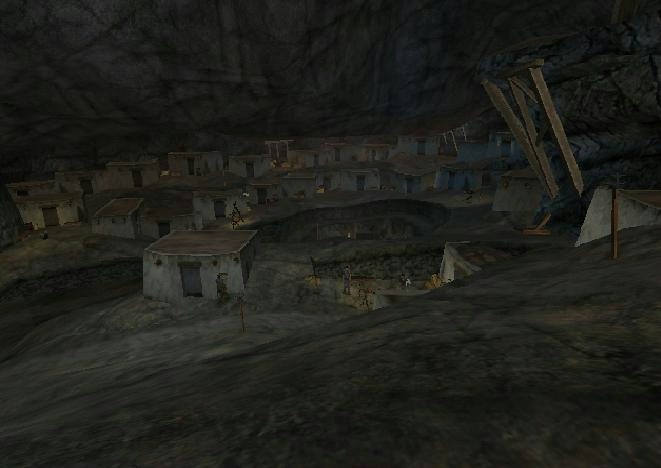
\includegraphics[scale=0.5]{nowyoboz.jpg}
\end{center}
Założony przez kilku ludzi, między innymi Lee i Laresa. Lee wyruszył z magami wody i założył obóz w górach na zachodzie. Tam powstała kontrolowana przez ten obóz Wolna Kopalnia. Magowie zamierzali użyć magicznej energii czystej rudy, by wysadzić barierę w powietrze. Niestety obóz ten nie handluje żadnym wartościowym towarem, jedynym jest wytwarzana tam gorzałka – ryżówka. Jednak większość mieszkańców kolonii uważa ją za paskudną, więc ma małą wartość. Dlatego Nowy Obóz kradnie dobra wysyłane Staremu Obozowi z kopalni.
Dzwięki w danej lokacji powinny powodować u gracza poczucie spokoju.
\section{Obóz na bagnie}
\begin{center}
 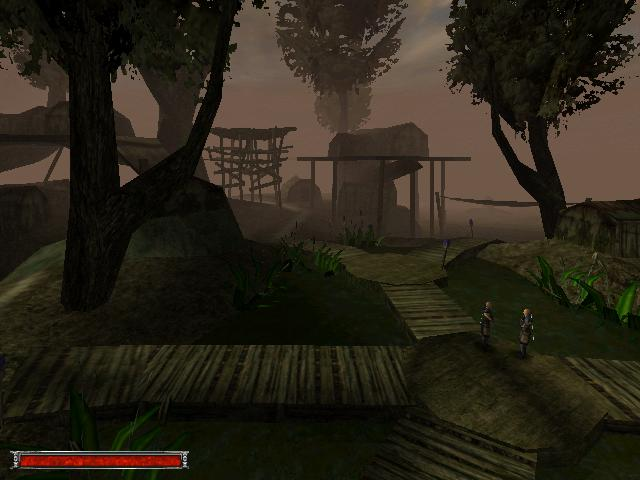
\includegraphics[scale=0.5]{nabagnie.jpg}
\end{center}
Stworzony przez jaśnie oświeconego Y'Beriona pięć lat przed sagą. Y'Berion otrzymał wizję od bóstwa zwanego Śniącym, które obiecało mu wskazanie drogi do wolności. Y'Berion usłuchał głosu Śniącego i zebrał wyznawców, którzy osiedlili się na bagnie na wschodzie, zakładając obóz bractwa zwanego też obozem na bagnie lub obozem sekty. Ludzie, którzy w nim mieszkali, nie musieli wydobywać rudy pod ziemią, gdyż obóz utrzymywał się ze sprzedaży innym obozom bagiennego ziela. Modlili się oni do Śniącego, by dał im wolność i szykowali się do wielkiego przywołania, które miało obudzić śpiące bóstwo.
Udzwiękowienie lokacji powinno budzić u gracza lekki niepokój oraz odzwierciedlać tajemniczość danego miejsca.
\section{Plac wymian}
\begin{center}
 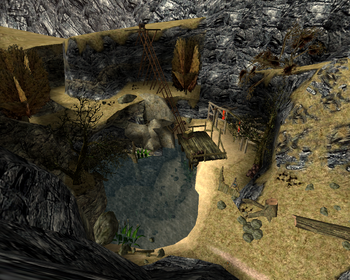
\includegraphics[scale=0.8]{placwymian.png}
\end{center}
Plac wymian za czasów magicznej bariery jest jedynym miejscem wymiany handlowej między królem a skazańcami ze Starego Obozu. Więźniowie wymieniają magiczną rudę na kobiety i towary z zewnętrznego świata, przewożone są za pomocą specjalnej platformy, obsługiwanej jedynie od góry. Na pośrednim klifie poza barierą są odczytywane wyroki dla skazańców, a następnie zostają oni zrzuceni do niewielkiego jeziorka, znajdującego się obok punktu wymian. Właśnie w tym jeziorku Bullit z kilkoma innymi strażnikami przeprowadza tak zwany „Chrzest wody”, polegający na uderzeniu żółtodziobów pięścią w twarz. Tutaj Bezimienny rozpoczyna swoją przygodę i odnajduje swoją pierwszą bryłkę magicznej rudy. Drogi ze Starego obozu, do placu wymian pilnuje Orry, razem ze swym strażnikiem.
Dzwieki zależne od sytuacji w jakiej gracz sie znajdzie w danej lokacji jeśli bedzie to walka to dzwięki muszą powodować u gracza niepokój a gdy gracz zwiedza lokacje powinny być to dzwięki natury.
\section{Opuszczona kopalnia}
\begin{center}
 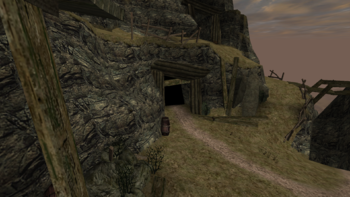
\includegraphics[scale=1.0]{opuszczonakopalnia.png}
\end{center}
 Jedna z kopalni w Górniczej Dolinie, znajdująca się przy drodze z placu wymian do Starego Obozu. Jest pierwszą kopalnią, z której wydobywano rudę. Po wielkim buncie została wcielona do Starego Obozu. Jest od dawna nieużywana z powodu wypadku, jaki się tam zdarzył. Od kopacza Grimesa ze Starej Kopalni, Bezimienny dowiaduje się, że powodem zawalenia się kopalni było pęknięcie podpór. Wokół niej można znaleźć kilof i pałkę oraz kilka innych przedmiotów, które prawdopodobnie pozostawili po sobie uciekający kopacze. Tereny wokół kopalni zamieszkują młode ścierwojady i młode kretoszczury.
 Dzwięki danej lokacji powinny budzic niepokój oraz tajemniczość u graczy.
\section{Wieża Xardasa}
\begin{center}
 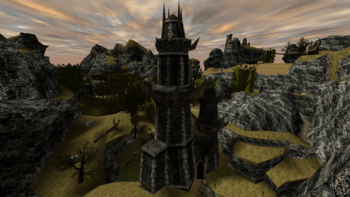
\includegraphics[scale=1.0]{wiezaxardasa.png}
\end{center}
Xardas wzniósł ją po zniszczeniu poprzedniej wieży z pomocą służących mu ożywieńców. Droga do wieży jest bardzo ciężka i pełna niebezpieczeństw. Dostać się do niej można idąc przez wąski wąwóz, który broniony jest przez kamiennego golema, lodowego golema oraz ognistego golema (sposób ich pokonania zawarty jest w księgach z cyklu Arcanum Golum). Wieża ma dwa piętra. Na parterze mieszczą się dwa pomieszczenia: w mniejszym nekromanta przechowuje swoje rzeczy, a większe zajęte jest przez jego sługę – demona. Na kolejne piętra można się dostać tylko dzięki runie teleportacyjnej, którą oprócz nekromanty posiada jedynie demon. Przekazuje on ją temu, kto pokona trzy golemy i przyniesie ich serca. Teleport prowadzi na pierwsze piętro do głównego pomieszczenia. Idąc korytarzem, można się dostać do małego pokoju, gdzie do ściany przybita jest drabina prowadząca na wyższą kondygnację. Tam też znajduje się siedziba Xardasa. Wokół stoją regały z książkami oraz stara makieta.
Udzwiękoienie danej lokacji powinny budzic niepokój u graczy.
\section{Zatopiona wieża Xardasa}
\begin{center}
 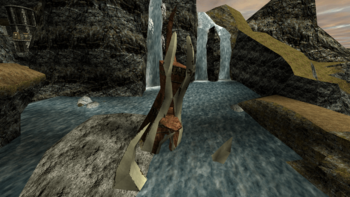
\includegraphics[scale=1.0]{zatopionawiezaxardasa.png}
\end{center}
Wieża znajduje się między starą cytadelą a górską fortecą. Xardas wzniósł ją zaraz po odejściu ze starego obozu. W wieży znajdowały się dwa obszerne, koliste pomieszczenia. Xardas przechowywał tam wszystko, co miał. Najcenniejsza była starożytna zbroja runiczna, którą nosił niegdyś wielki generał. Został on jednak zabity przez orków. Nie wiadomo, w jaki sposób nekromanta wszedł w posiadanie pancerza. Podczas jednego z trzęsień ziemi wody pobliskiego jeziora zalały imponującą budowlę. Uratował się tylko nekromanta. Wodą nie zostały zalane dwa pokoje, które zostały zajęte przez zombie i szkielety.
Dzwięki danej lokacji powinny budzic niepokój oraz tajemniczość u graczy.
\section{Miasto Orków}
\begin{center}
	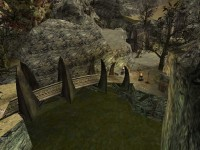
\includegraphics[scale=1.8]{miastoorkow.jpg}
\end{center}
Prymitywna osada plemienia Orków. Aby móc poruszać się po Mieście Orków bez obaw o życie, należy mieć ze sobą symbol pokoju – dwuręczną broń zwaną Ulu-Mulu. Pod miastem znajduje się Świątynia Śniącego.
Dzwięki danej lokacji powinny budzic niepokój u graczy.
\section{Stara kopalnia}
\begin{center}
	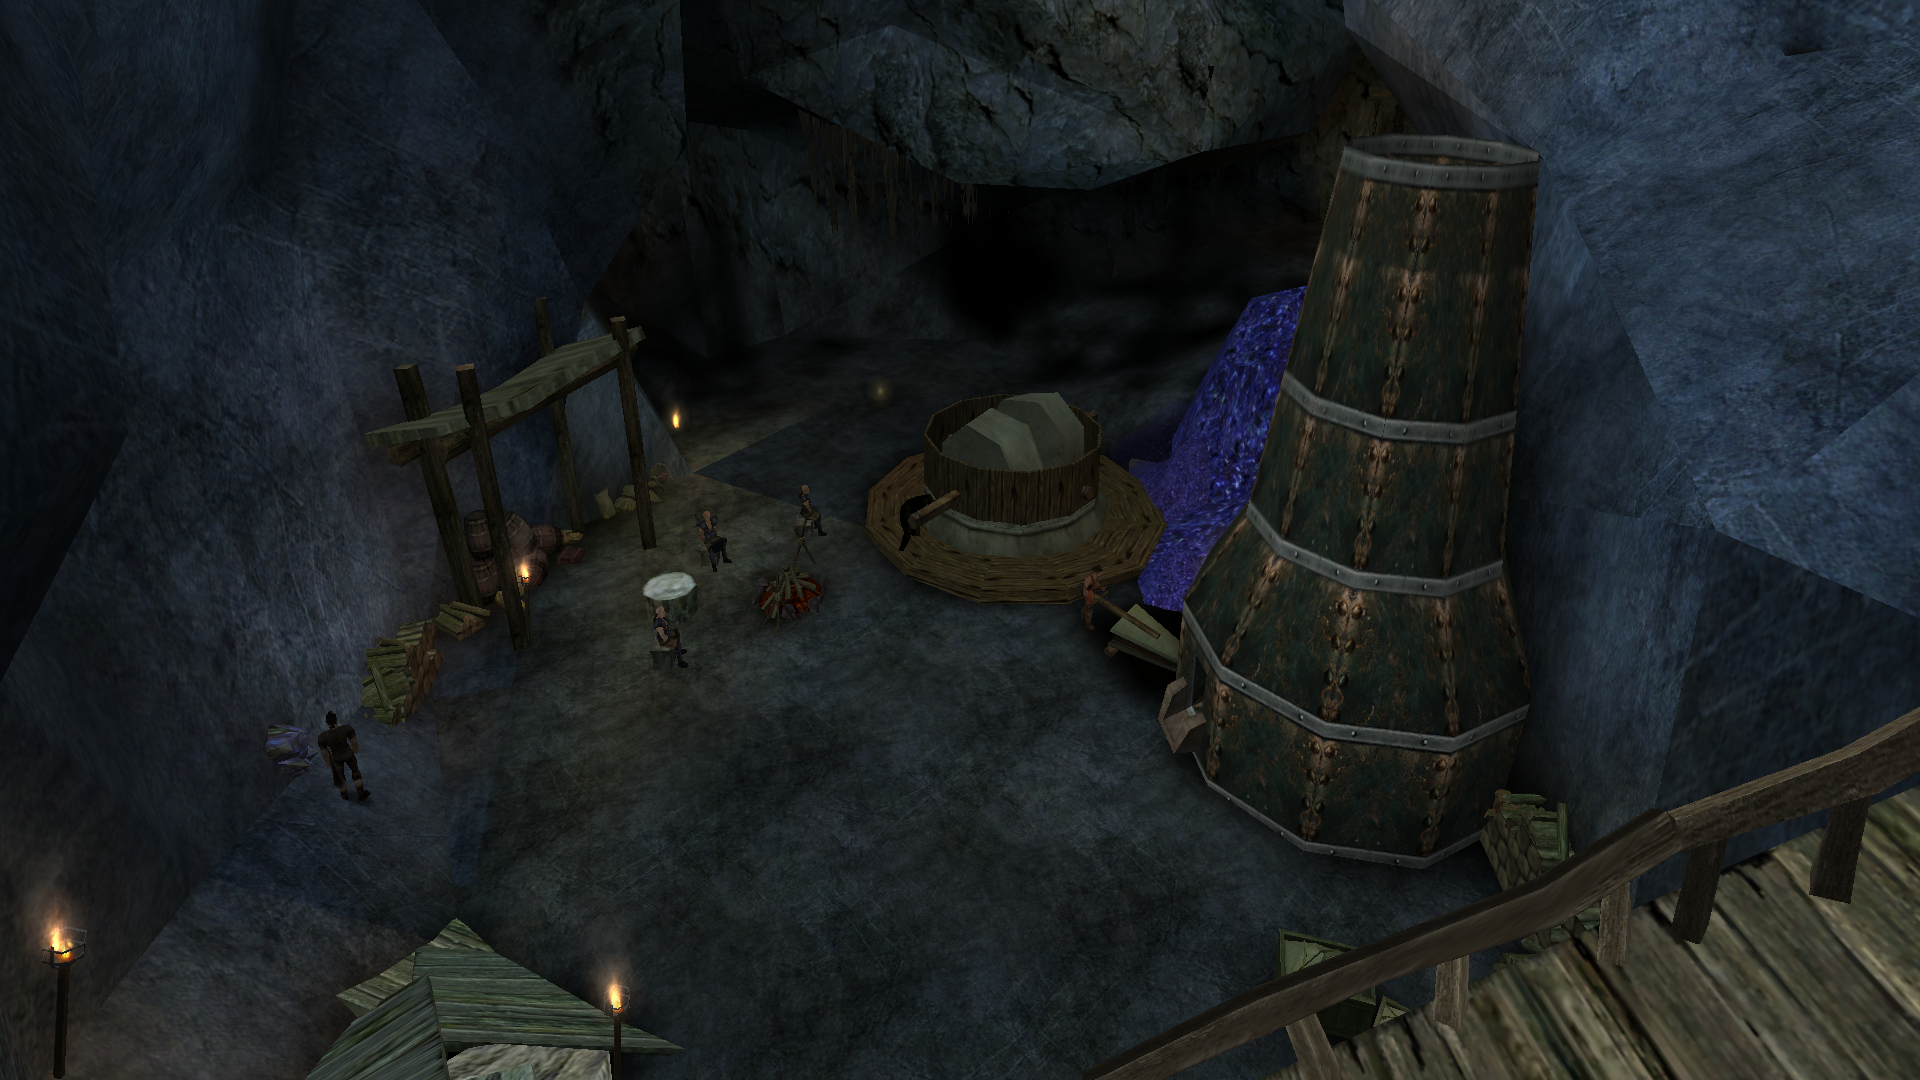
\includegraphics[scale=0.25]{twojastara-kopalnia}
\end{center}
W kopalni jest wydobywana ruda dla króla. Co miesiąc kopacze wykopują dwieście worków dla Rhobara, a kolejne dwadzieścia worków jest od razu przetapiane. W kopalni głównym problemem są pełzacze, które uniemożliwiają wydobycie rudy w niektórych jaskiniach. Mimo że te stawonogi są tępione przez strażników świątynnych, ich populacja wciąż się zwiększa przez ich królową. W kopalni znajdują się dwaj handlarze – Santino, który znajduje się niedaleko wyjścia oraz Alberto, który przebywa niedaleko Iana. Oferują oni jedzenie, strzały, bełty i mikstury lecznicze. W kopalni jest także magazyn pilnowany przez kwatermistrza Ulberta. Jeśli Bezimienny chce zostać członkiem Starego lub Nowego Obozu, musi odebrać od Iana listę dla Diego, w której wypisane są rzeczy potrzebne dla ludzi z kopalni. W drugim rozdziale bohater na zlecenie Cor Kaloma musi odnaleźć jaja pełzaczy. Po załatwieniu koła zębatego dla Iana i wsparcia dla Asghana udaje mu się osiągnąć cel.
Dzwięki danej lokacji powinny budzic niepokój oraz informować gracza o grasującym tam niebezpieczeństwie.
\section{Stary klasztor}
\begin{center}
	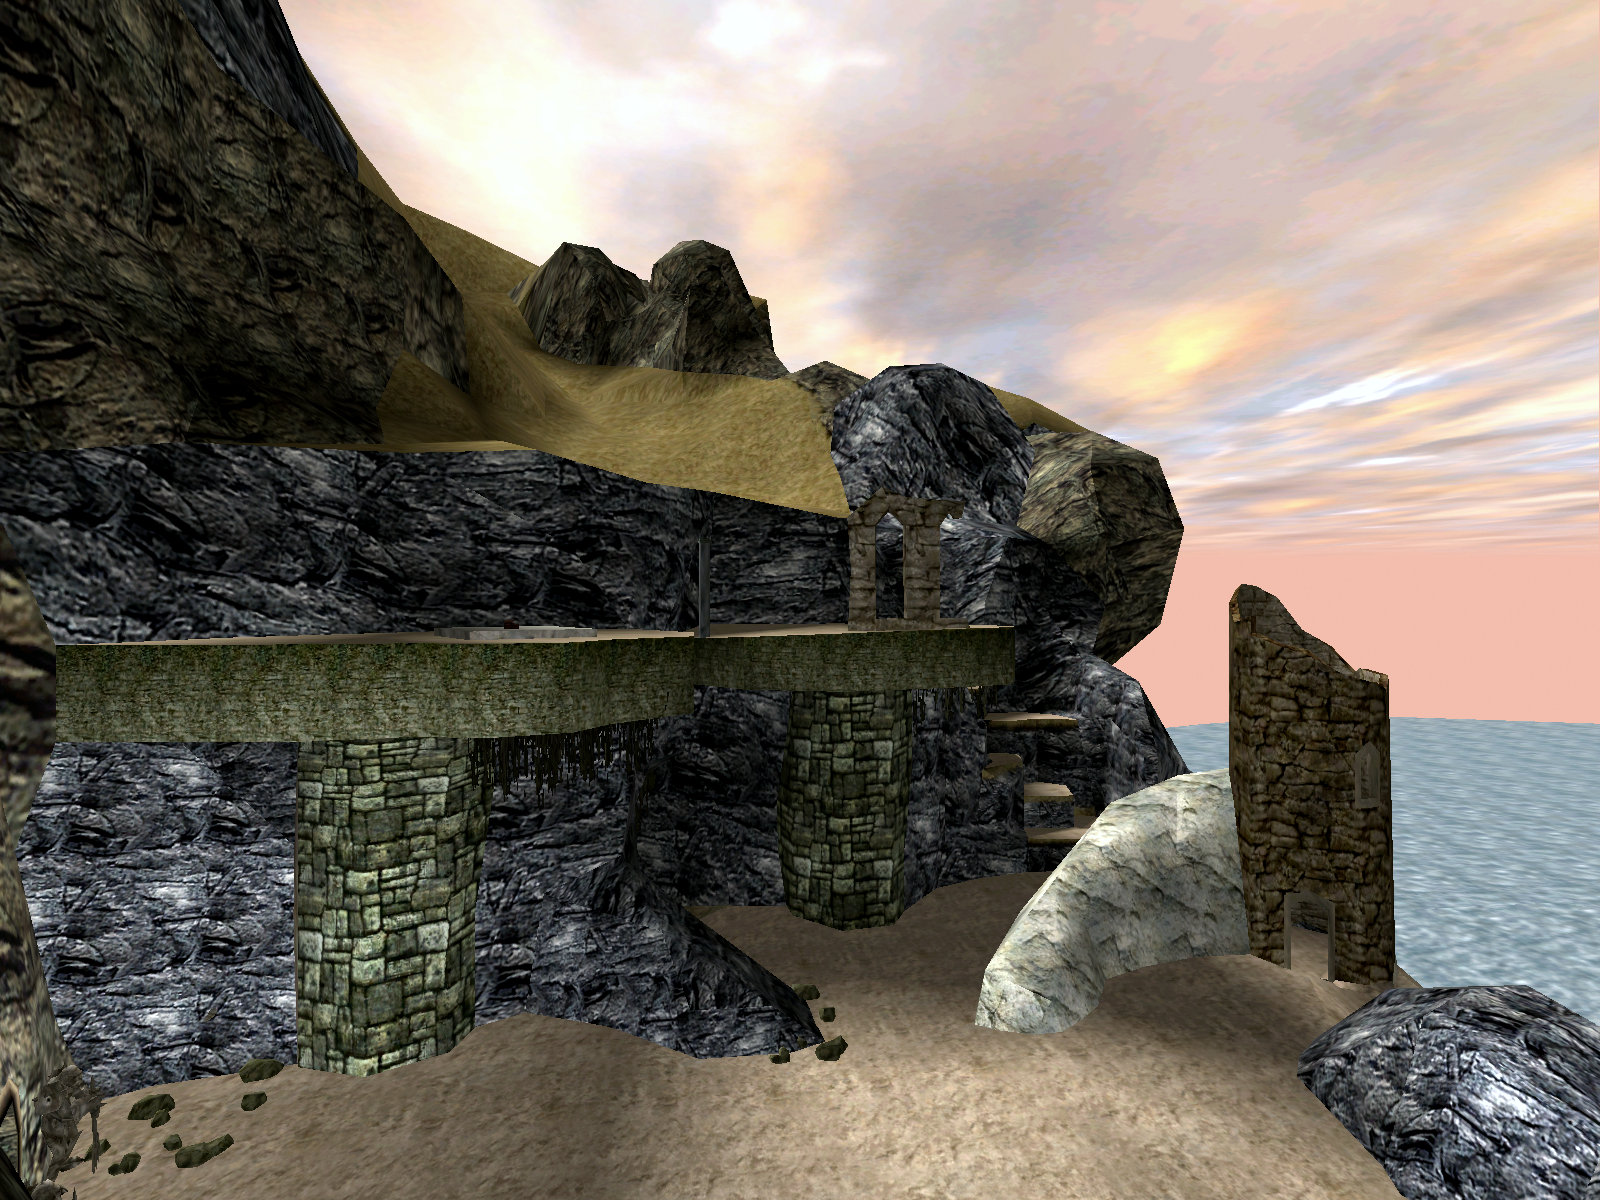
\includegraphics[scale=0.25]{twojastara-klasztor}
\end{center}
Pozostałości po nieznanym kataklizmie. Wewnątrz nie znajduje się nic oprócz kilku zębaczy, cieniostwora i młodego trolla. Przez to, że brama jest zamknięta od środka, dostać się tam można tylko dzięki przemianie w chrząszcza i przejściu przez małą szczelinę w murze. Bezimienny wraz z Gornem znajdują tutaj jeden z pięciu kamieni ogniskujących, potrzebnych Magowi Wody, Saturasowi. Niewykluczone, że druidzi opuścili klasztor i wyruszyli do Myrtany.
Dzwięki danej lokacji powinny budzic niepokój u graczy.
\section{Swiątynia śniącego}
\begin{center}
	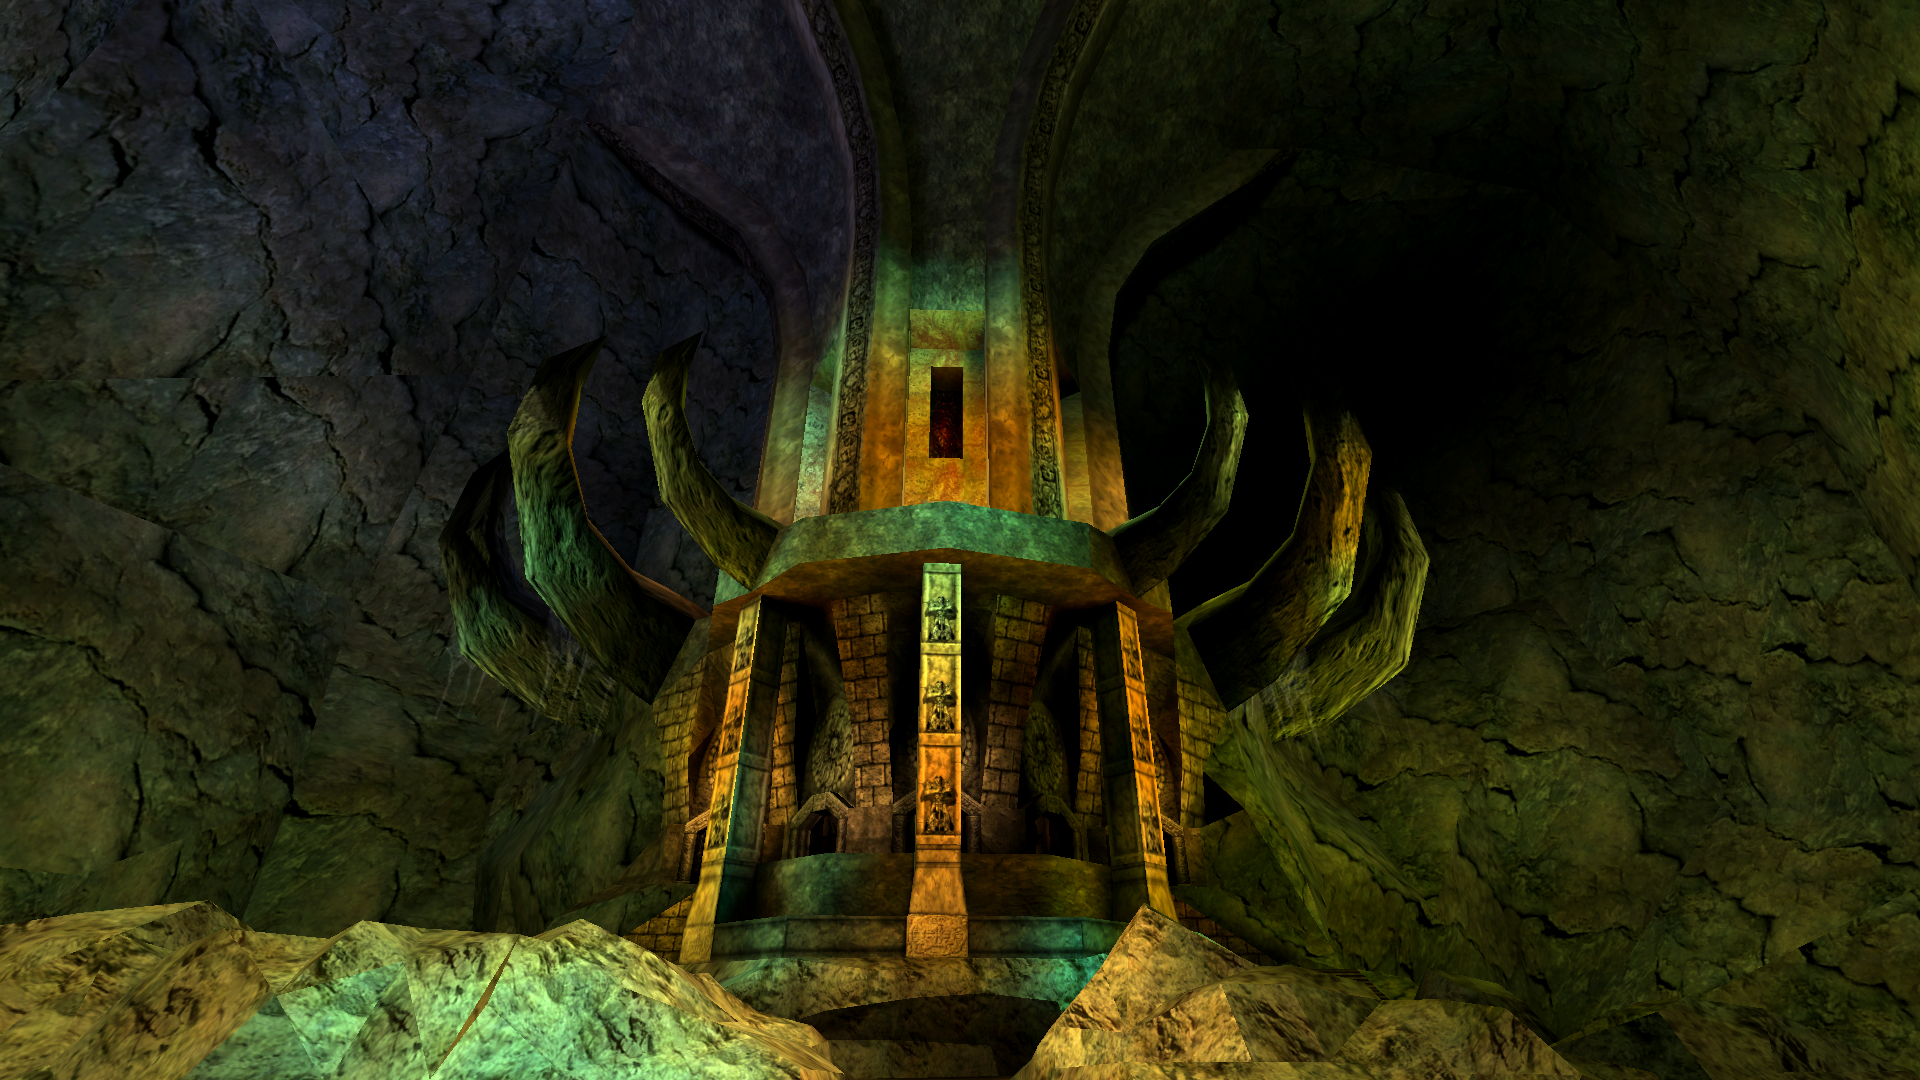
\includegraphics[scale=0.25]{swiatyniasniacego}
\end{center}
Tysiąc lat przed wydarzeniami z Gothic orkowi szamani przywołali potężnego demona. Nazwali go Krushak. Pokonał on wrogie im klany, a w podzięce orkowie wnieśli mu olbrzymią, wspaniałą świątynię. Budowla była pełna przeróżnych pułapek i ślepych uliczek. Demon jednak zamiast być wdzięcznym wyrwał serca pięciu orkowym kapłanom i zamienił wszystkich w ożywieńców. Taki sam los spotkał budowniczych świątyni. Przerażeni orkowie zamknęli wejście do świątyni i uśpili demona. Składali mu ofiary, by go przebłagać. W Świątyni Orkowie schowali miecz pokonanego przez nich wojownika, niegdyś generała w wojnie z orkami – Uriziela. Tysiąc lat później Cor Kalom i jego poplecznicy wyruszyli do świątyni, aby przebudzić demona. Za nimi poszedł Bezimieny. Wybraniec Innosa pokonał szamanów, hordy ożywieńców, apokaliptycznych strażników świątynnych i samego guru. Potem przebił serca kapłanów ich mieczami i Śniący został wygnany do Wymiaru Beliara. Świątynia zawaliła się, a wraz z nią pogrzebany został Bezimienny.
Dzwięki danej lokacji powinny budzic niepokój oraz informować gracza o grasującym tam niebezpieczeństwie.
\section{Obóz bandytów}
\begin{center}
	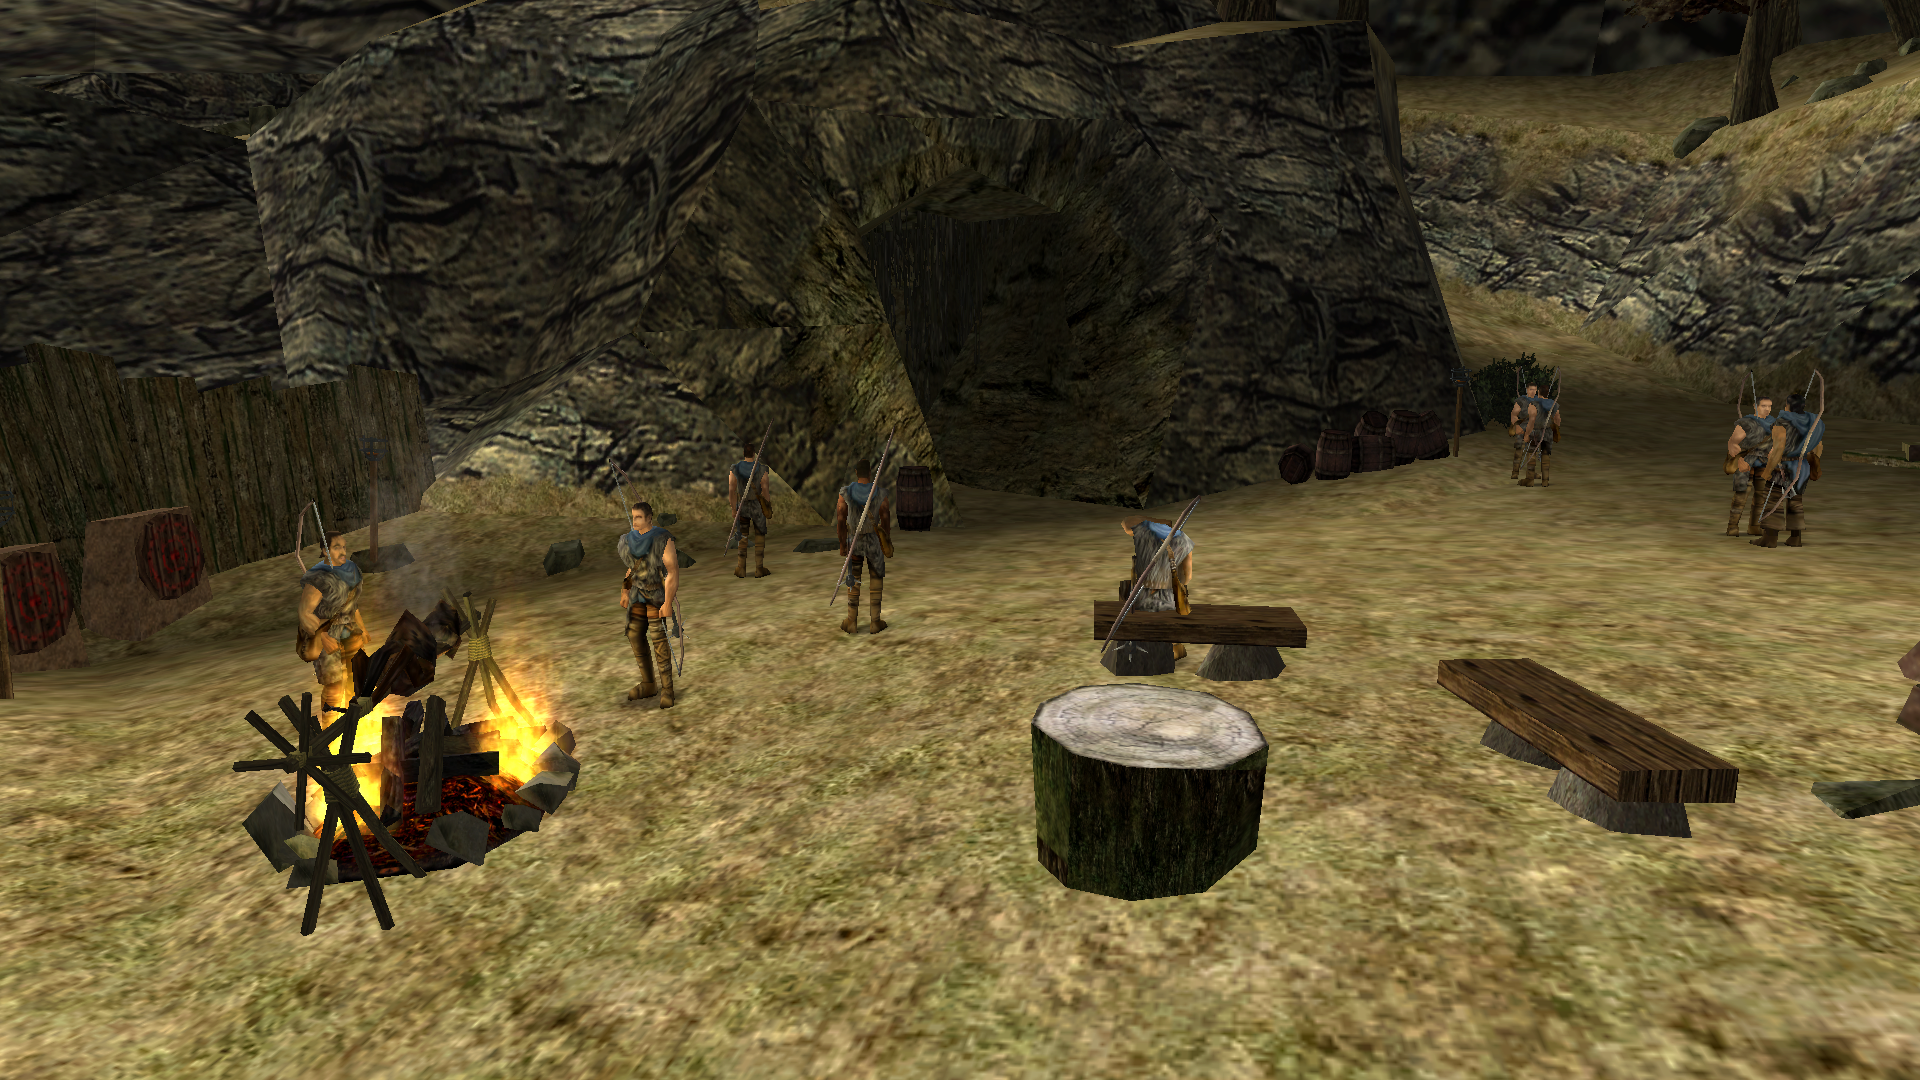
\includegraphics[scale=0.25]{obozbandytow}
\end{center}
Niewielki obóz, w którym mieszkają bandyci pod przywództwem Quentina. Ubiór bandytów może sugerować, że są oni uciekinierami z Nowego Obozu. Obóz znajduje się wewnątrz gór, niedaleko Kanionu trolli. Ze względu na swoje położenie ma duże właściwości obronne i ciężko go wykryć.
Dzwięki danej lokacji powinny budzic niepokój, informować gracza o grasującym tam niebezpieczeństwie oraz 
przygotowywać do walki.
\chapter{Projektowanie postaci}\label{chapt:model}
\section{Podstawowe informacje}
W grze Gothic gracz wciela się w postać zwaną Bezimiennym tj. Rhobar III. Jest to wybraniec bogów oraz główny protagonista serii Gothic. Jest młodym, dobrze zbudowanym mężczyzną, ma wąsy i małą bródkę, piwne oczy, włosy ciemnoblond zebrane z tyłu w niewielki kucyk. Wykazuje często ironiczne poczucie humoru, niekiedy autoironiczne, choć ma jednocześnie poczucie swojej wartości i bywa wrażliwy na punkcie godności osobistej. W fabule gry nie zostało powiedziane, za jakie przestępstwo został zesłany do Górniczej Doliny, wiadomo tylko tyle, że zanim tam trafił, przesiedział dwa miesiące w lochu. Jako twórcy dopiero w 3 części gry powiemy, że został zesłany do kolonii, by odkrył swoją moc, i że jest wybrańcem. Bohater nie został również przedstawiony z imienia – choć w trakcie gry kilka razy bezskutecznie usiłuje się sam przedstawić.
\begin{center}
	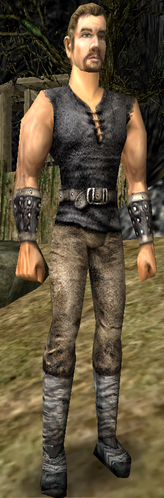
\includegraphics[scale=0.6]{bezi.png}
\end{center}
\section{Historia, i fabuła związna z protagonistą}
Bezimienny trafia do Górniczej Doliny, która dekretem króla Myrtany stała się kolonią karną. Chwilę przed skazaniem dostaje list od arcymistrza ognia – Pyrokara, który ma dostarczyć magom ognia spod bariery. Zaraz po zrzuceniu zostaje „powitany” przez Bullita. Z tarapatów ratuje go przywódca cieni – Diego, który przepędza bandę. Diego staje się też przewodnikiem Bezimiennego w kolonii, a także jego pierwszym przyjacielem. Podczas podróżowania po kolonii, główny bohater zaprzyjaźnia się także z Miltenem, Lesterem i Gornem. Ostatecznie dostarcza list od Pyrokara magom ognia.

Słysząc o jego dokonaniach najwyższy guru w Obozie Bractwa – Y'Berion pragnął z nim porozmawiać. Kiedy doszło do spotkania, Mistrz mówi, że kiedyś się już spotkał z Bezimiennym, jednak ten zaprzecza. Na polecenie Y'Beriona udaje się na poszukiwania kamienia ogniskującego. Cor Kalom zleca mu przyniesienie starożytnego Almanachu oraz jaj pełzaczy. Gdy zabija królową pełzaczy w Starej Kopalni, zostaje nagrodzony i awansuje. Jego dokonania doprowadzają do wielkiego przywołania. Po tym, jak Y'Berion został osłabiony, a oddział straży świątynnej nie wracały długo z cmentarzyska orków, Cor Angar wysyła tam Bezimiennego. Na cmentarzu okazało się, iż w wyniku napaści orków zabici zostali wszyscy ludzie z ekspedycji Bractwa z wyjątkiem Baala Lukora. Z pomocą Bezimiennego guru zagłębia się w starożytnych zapiskach na grotach, aż w końcu, nic nie znajdując, rzuca się na niego. Bohater, pokonawszy opętanego guru, wraca do Obozu Bractwa, gdzie od Cor Angara dowiaduje się, że Wielki Mistrz umiera. Nawet nazbierane przez Bezimiennego zioła uzdrawiające z wielkiego bagna nie pomogły Y'Berionowi. Na dodatek okazało się, iż Śniący jest prastarym demonem. Dowiedziawszy się o tym asystent Mistrza – Cor Kalom, zebrał grupę ludzi, która nadal wierzyła w Śniącego i opuścili Obóz Bractwa, poszukując go na własną rękę. Cor Angar wysyła Bezimiennego do magów wody, informując go, że Y'Berion przed śmiercią pokładał nadzieje w ich planie ucieczki.

Zgodnie z wolą Cor Angara, Bezimienny udaje się do Nowego Obozu, gdzie rezydują magowie wody. Arcymag wody – Saturas planował zniszczyć barierę poprzez wysadzenie wielkiego kopca rudy. Kiedy rudy było już wystarczająco dużo, magowie postanowili wysłać Bezimiennego, aby znalazł kamienie ogniskujące, żeby magowie mogli zogniskować moc w nich zawartą do kopca rudy. Bezimienny z pomocą swych przyjaciół zdołał zebrać wszystkie kamienie. Pokonał także ich strażników: harpie, szkielety, trolla, gobliny, zębacze oraz Nadzorcę. Gdy misja została wykonana, zanosi kamienie Saturasowi, który poprosił go o pójście do magów ognia i nakłonienie ich do udziału w rytuale wysadzenia rudy. Niestety będąc na miejscu, Bezimienny dowiaduje się od swojego przyjaciela Miltena, że magowie ognia zostali wymordowani, a Stara Kopalnia się zawaliła. Diego dodał, że strażnicy magnatów pomaszerowali ku Wolnej Kopalni, aby ją zdobyć. Dodatkowo strażnicy Gomeza uważają Bezimiennego za zdrajcę, gdyż ten pomagał Nowemu Obozowi.

Na wieść o śmierci magów ognia Saturas prosi Bezimiennego o odnalezienie potężnego nekromanty – Xardasa. Bezimienny zdołał odnaleźć wieżę maga i dzięki pokonaniu trzech golemów, dostaje się do niego za pomocą runy, którą podarował mu Demon Ognia. Xardas wyjaśnia, że wysadzenie kopca rudy nie zniszczy bariery. Jedynym sposobem na pokonanie tego czaru jest magia demonów. Należy wygnać ze świata mrocznego demona – Śniącego. Opowiada Bezimiennemu część historii Śniącego. Aby dowiedzieć się kolejnej części, Bezimienny musi udać się do cytadeli orków, gdzie przebywa wygnany szaman orków – Ur-Shak. Będąc na miejscu, okazało się, że Ur-Shak jest atakowany przez orkowych strażników. Bezimienny pomaga mu w walce, a następnie wysłuchuje resztę historii Śniącego. Dowiaduje się też, że aby dostać się bez walki do miasta orków, gdzie znajduje się świątynia demona, należy posiadać Ulu-Mulu. Bezimienny planuje udać się do zajętej przez straż Gomeza kopalni Nowego Obozu, gdzie przebywa orkowy niewolnik – Tarrok, który potrafi sporządzić tę przedziwną broń. Saturas nie był zadowolony z misji Bezimiennego, gdyż ten skłamał, że nie odnalazł Xardasa. Udaje się następnie wraz z Gornem do Wolnej Kopalni bronionej przez Szakala i jego ludzi. Z pomocą najemnika udało się oczyścić kopalnię, a następnie odnaleźć Tarroka. Ork mówi, że do sporządzenia Ulu-Mulu potrzebny jest: język ognistego jaszczura, kieł trolla, kły węża błotnego i róg cieniostwora. Po długich poszukiwaniach udało się odnaleźć wszystkie składniki. Bohater uzbrojony w Ulu-Mulu udaje się do miasta orków i wkracza do świątyni Śniącego. Eliminując kolejno najwyższych szamanów, nieumarłych i ludzi Cor Kaloma, odnajduje starożytny miecz Uriziel. Jakiś czas później staje oko w oko z ostatnim szamanem, który okazał się nieśmiertelny. Jedynym ratunkiem była ucieczka ze świątyni.

Bezimienny wraca prosto do wieży Xardasa, wyjaśniając mu tajemnicę ostatniego szamana i pokazując Uriziel. Nekromanta doszedł do wniosku, że tylko Uriziel jest w stanie pokonać nieśmiertelnego szamana. Niestety miecz będąc wiele lat w rękach orków, stracił swą moc. Aby go ponownie naładować, Xardas musi sporządzić magiczną formułę. W tym czasie Bezimienny udaje się do pierwszej wieży Xardasa, która wiele lat temu została zalana wodą. Odnajduje tam starożytną zbroję runiczną oraz teleport do Starego Obozu. Korzystając z runy teleportacji, udaje się do świątyni magów ognia. Wybijając kolejnych strażników, dostaje się do siedziby magnatów, gdzie zabija ich przywódcę – Gomeza. Dzięki kluczowi Gomeza dostaje się do lochów, gdzie przetrzymywany był kowal Stone. Wzmacnia on zbroję runiczną Bezimiennego. Bohater następnie wraca do wieży nekromanty, który zdołał przygotować już czar. Potrzeba było jeszcze wielkiej ilości energii oraz maga, który odczyta zaklęcie. Zgodnie z planem Bezimienny udaje się do Nowego Obozu. Jego przyjaciel – Milten zgadza się mu pomóc. Jest to ryzykowne, ponieważ bohater musi przelać na Uriziel energię z rudy magów wody, którą tak długo gromadzili. Podczas rytuału Bezimiennego nakryli go magowie – Saturas, Myxir oraz Riordian. Bohater ucieka z Nowego Obozu i udał się ponownie do świątyni Śniącego, gdzie zdołał pokonać ostatniego szamana.

Zabiwszy szamana, udaje się do następnej komnaty, gdzie niespodziewanie spotyka Xardasa. Nekromanta wyjaśnia, że aby zniszczyć barierę, należy wygnać Śniącego poprzez przebicie mieczami szamanów pięciu serc w kaplicach. Powiedziawszy to, mag stracił przytomność, a Bezimienny udaje się do głównej komnaty Śniącego. Okazało się, że szalony Kalom i jego ludzie zdołali obudzić demona. Mimo miotanych przez Śniącego ognistych kul Bezimienny pokonuje ludzi Bractwa i staje oko w oko z demonem. Za każdym razem, gdy przebija urnę z sercem szamana, pojawia się jego asystent – książę demonów. Dzięki Urizielowi udało mu się stawić czoło demonom i przebić wszystkie serca orkowych szamanów. Otworzył się ogromny portal prowadzący do wymiaru Beliara. Jednak Śniący ostatnim tchnieniem zdołał wezwać Siły Ciemności. Chwilę później demon zostaje wessany, a jego klęska sprawiła, iż upada bariera. Wskutek zniszczenia kopuły nad Górniczą Doliną pojawia się magiczna burza, a seria trzęsień wstrząsnęła ziemią. Świątynia Śniącego zawala się, przygniatając Bezimiennego. Jedynie magiczny pancerz ratuje go przed śmiercią.
\newline
\section{Mocne strony postaci}
 Wraz z rozwojem fabuły postac zyskuje na sile oraz walka z mobami jest coraz łatwiejsza.
 Rozwój postaci jest zależny od samego gracza ponieważ on decyduje jaką statystyke bohatera chce aktualnie rozwinąć.
\section{Słabe strony postaci}
Postać na samym początku rozgrywki jest bardzo słaba.
Gracz ma czuć progres wraz z rozwojem fabuły.
\section{Wygląd postaci}
\begin{center}
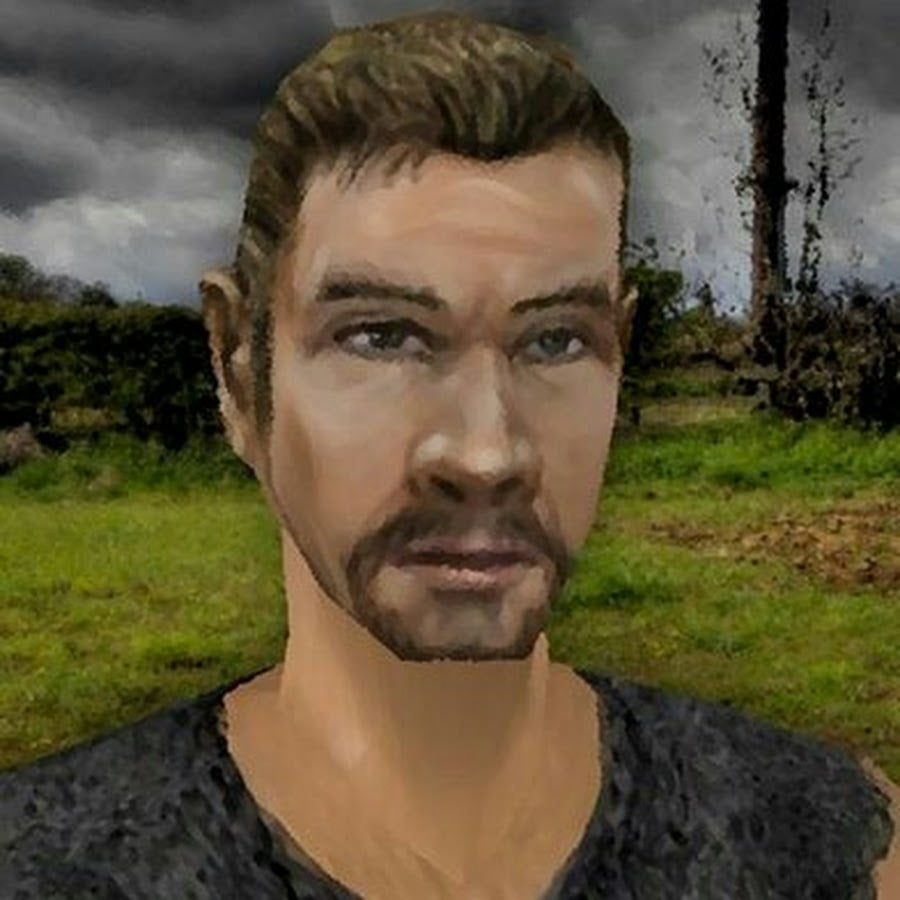
\includegraphics[scale=0.37]{bezimienny}
\end{center}
\begin{center}
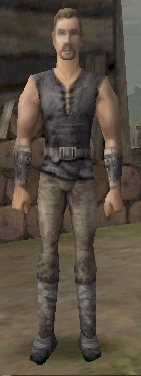
\includegraphics[scale=2]{bezzimiennybody}
\end{center}
\begin{center}
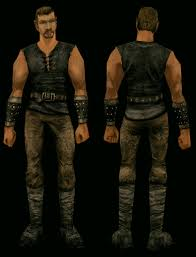
\includegraphics[scale=2]{bezimiennybody2}
\end{center}
\chapter{Flowboard}
\section{Rozdział 1 - Witamy w Kolonii!}
\begin{center}
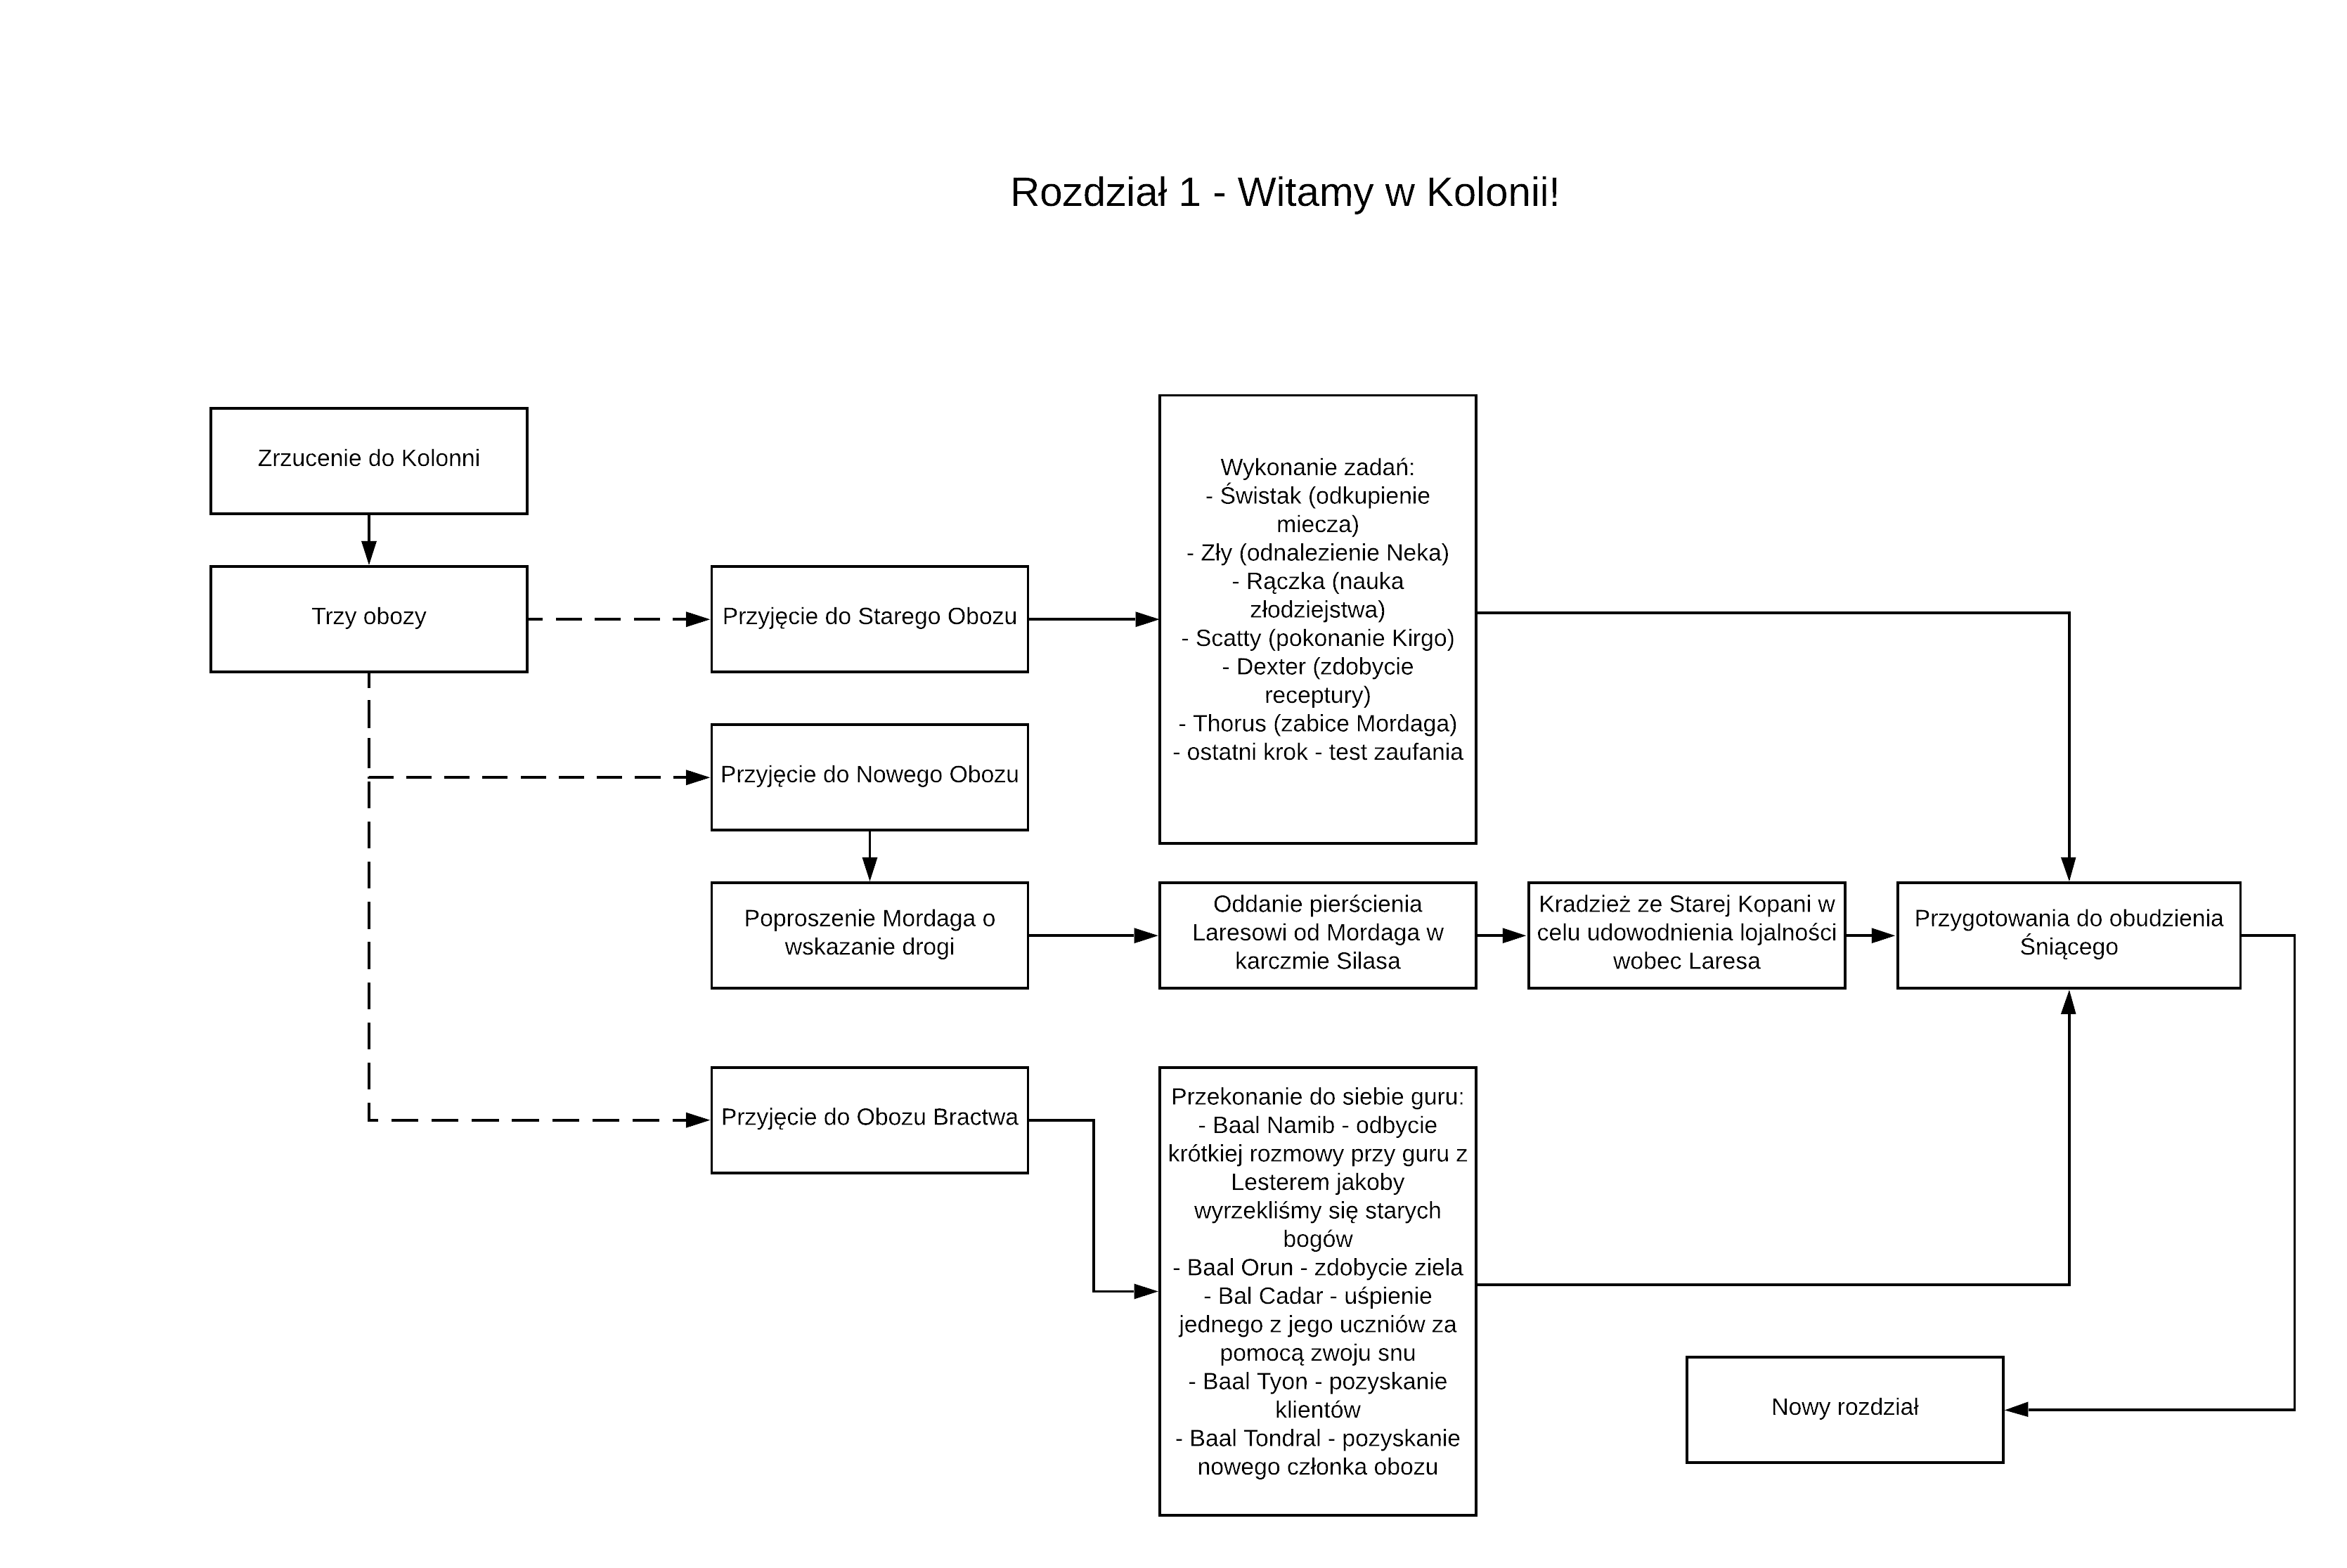
\includegraphics[scale=0.13, angle=90]{rozdzial1}
\end{center}
\section{Rozdział 2 - Gniazdo pełzaczy}
\begin{center}
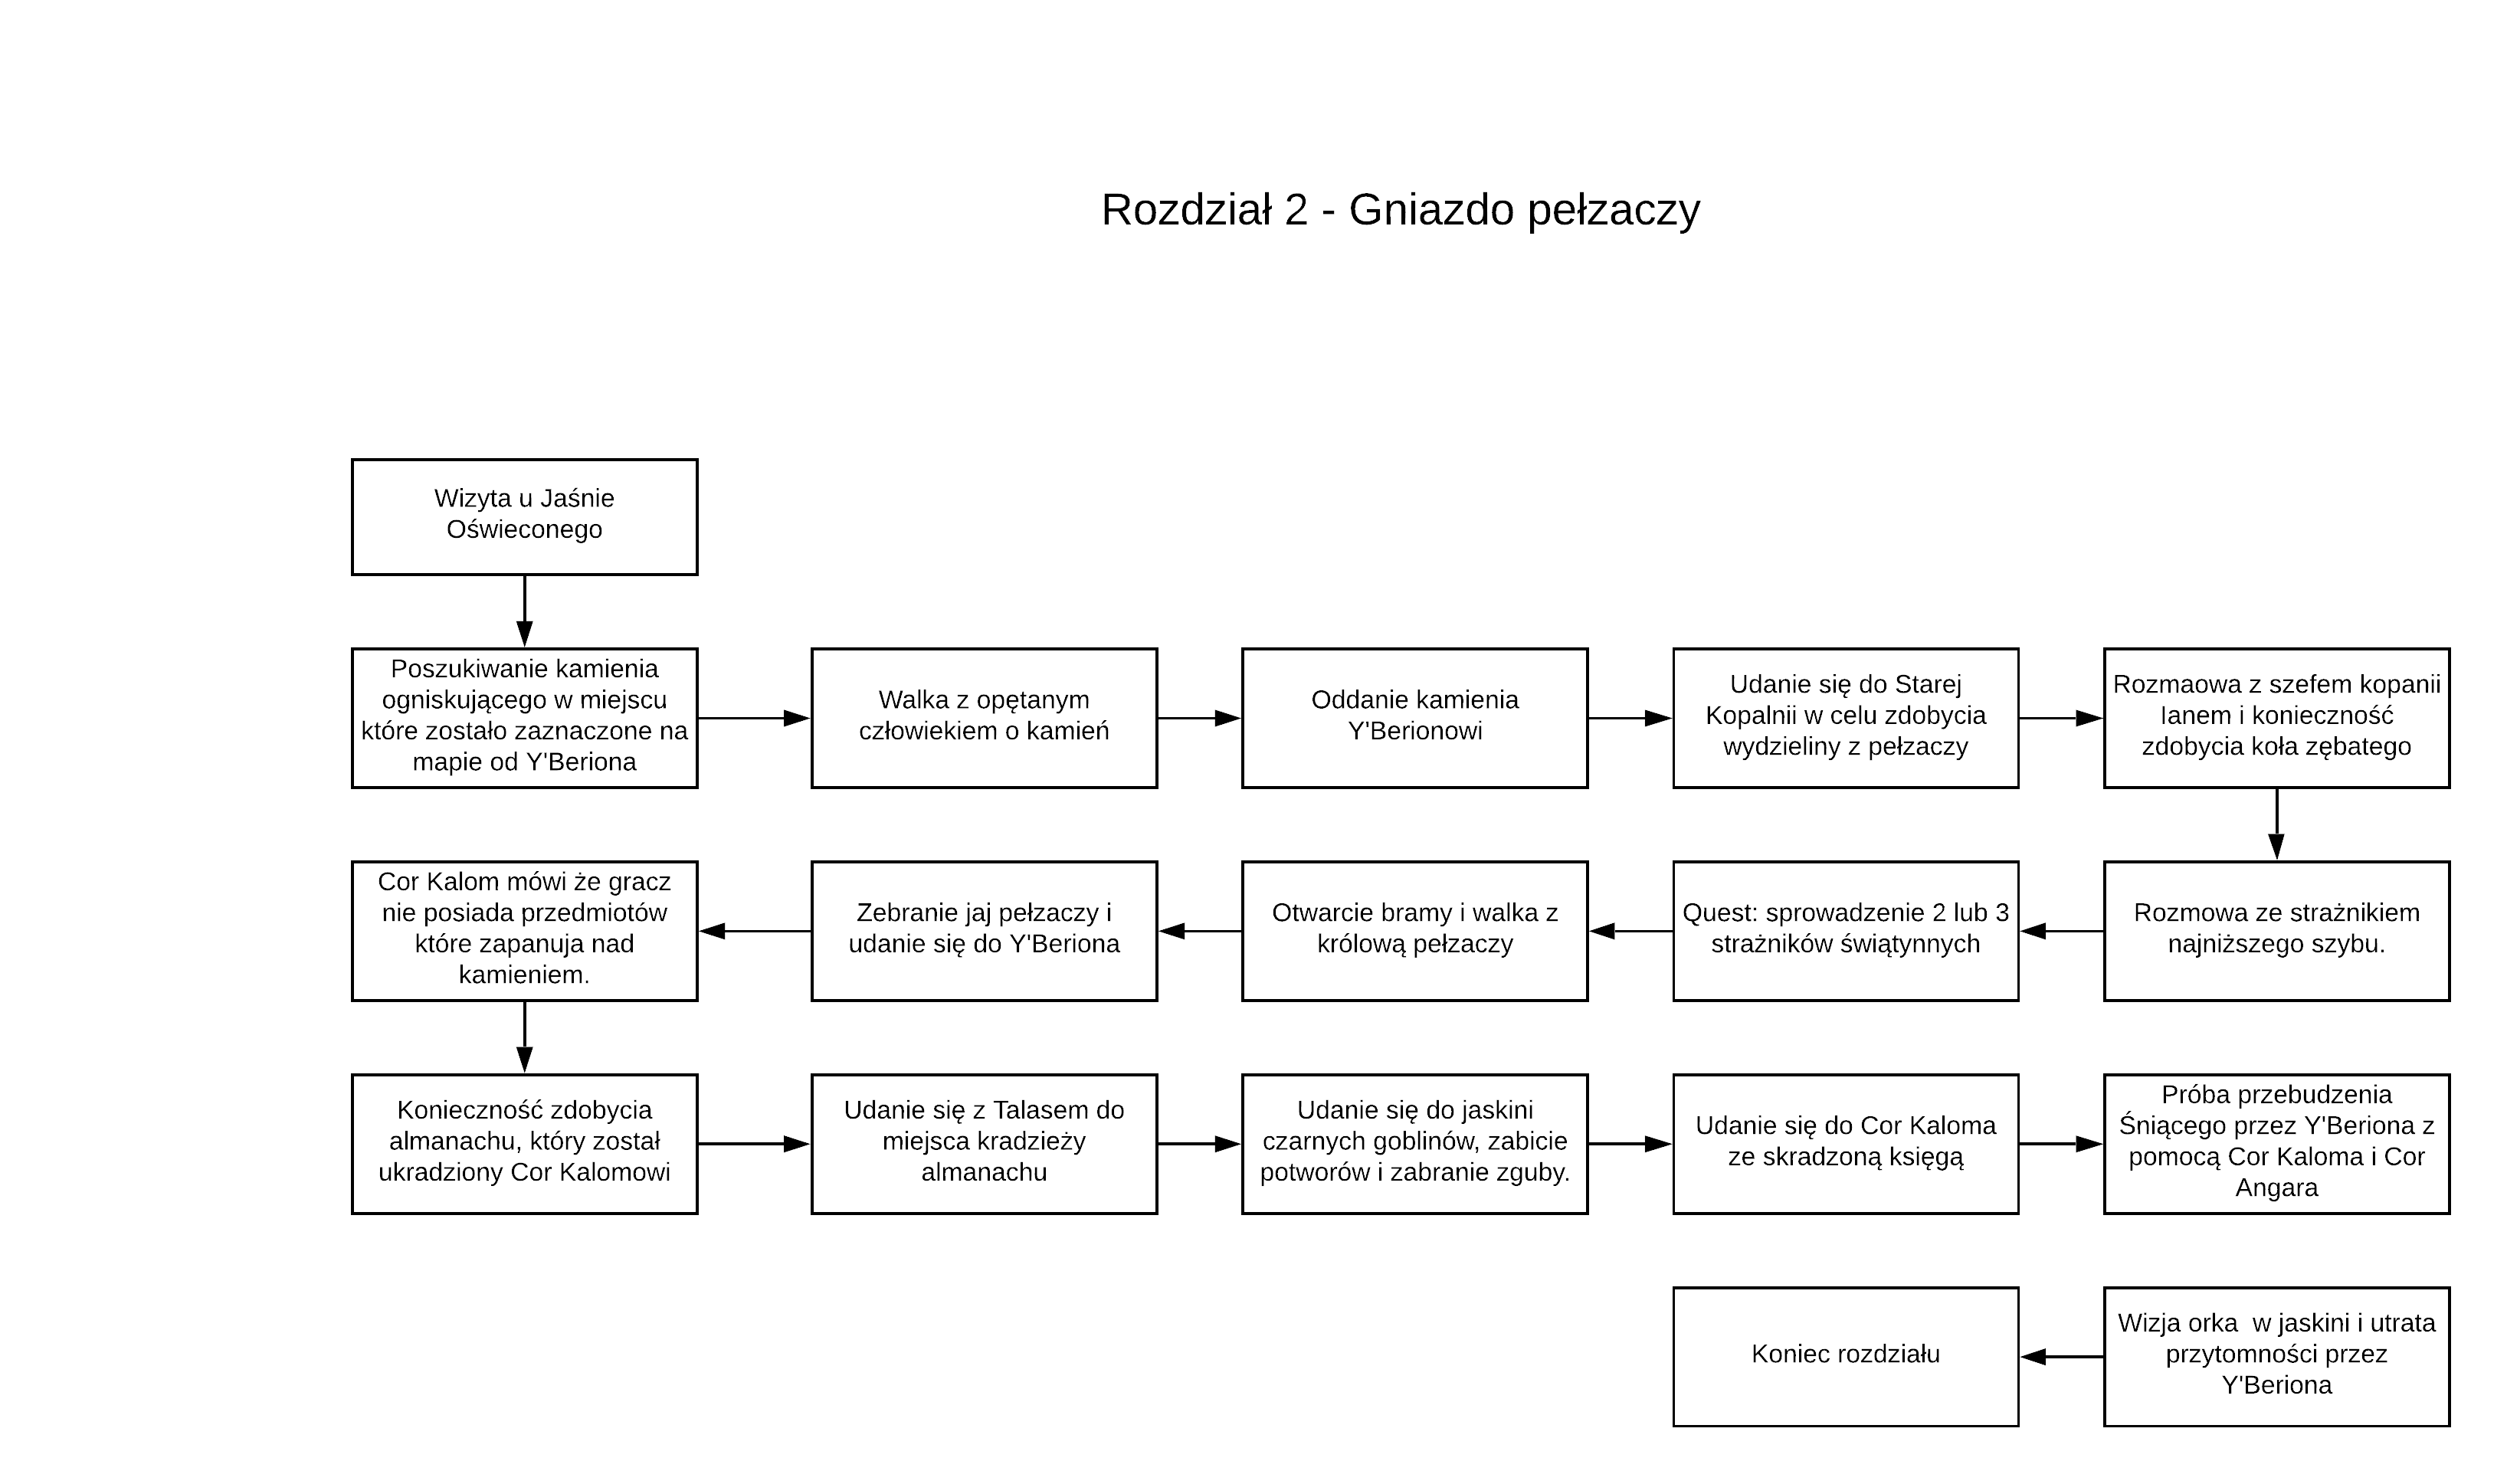
\includegraphics[scale=0.17, angle=90]{rozdzial2}
\end{center}
\section{Rozdział 3 - Starożytna magia}
\begin{center}
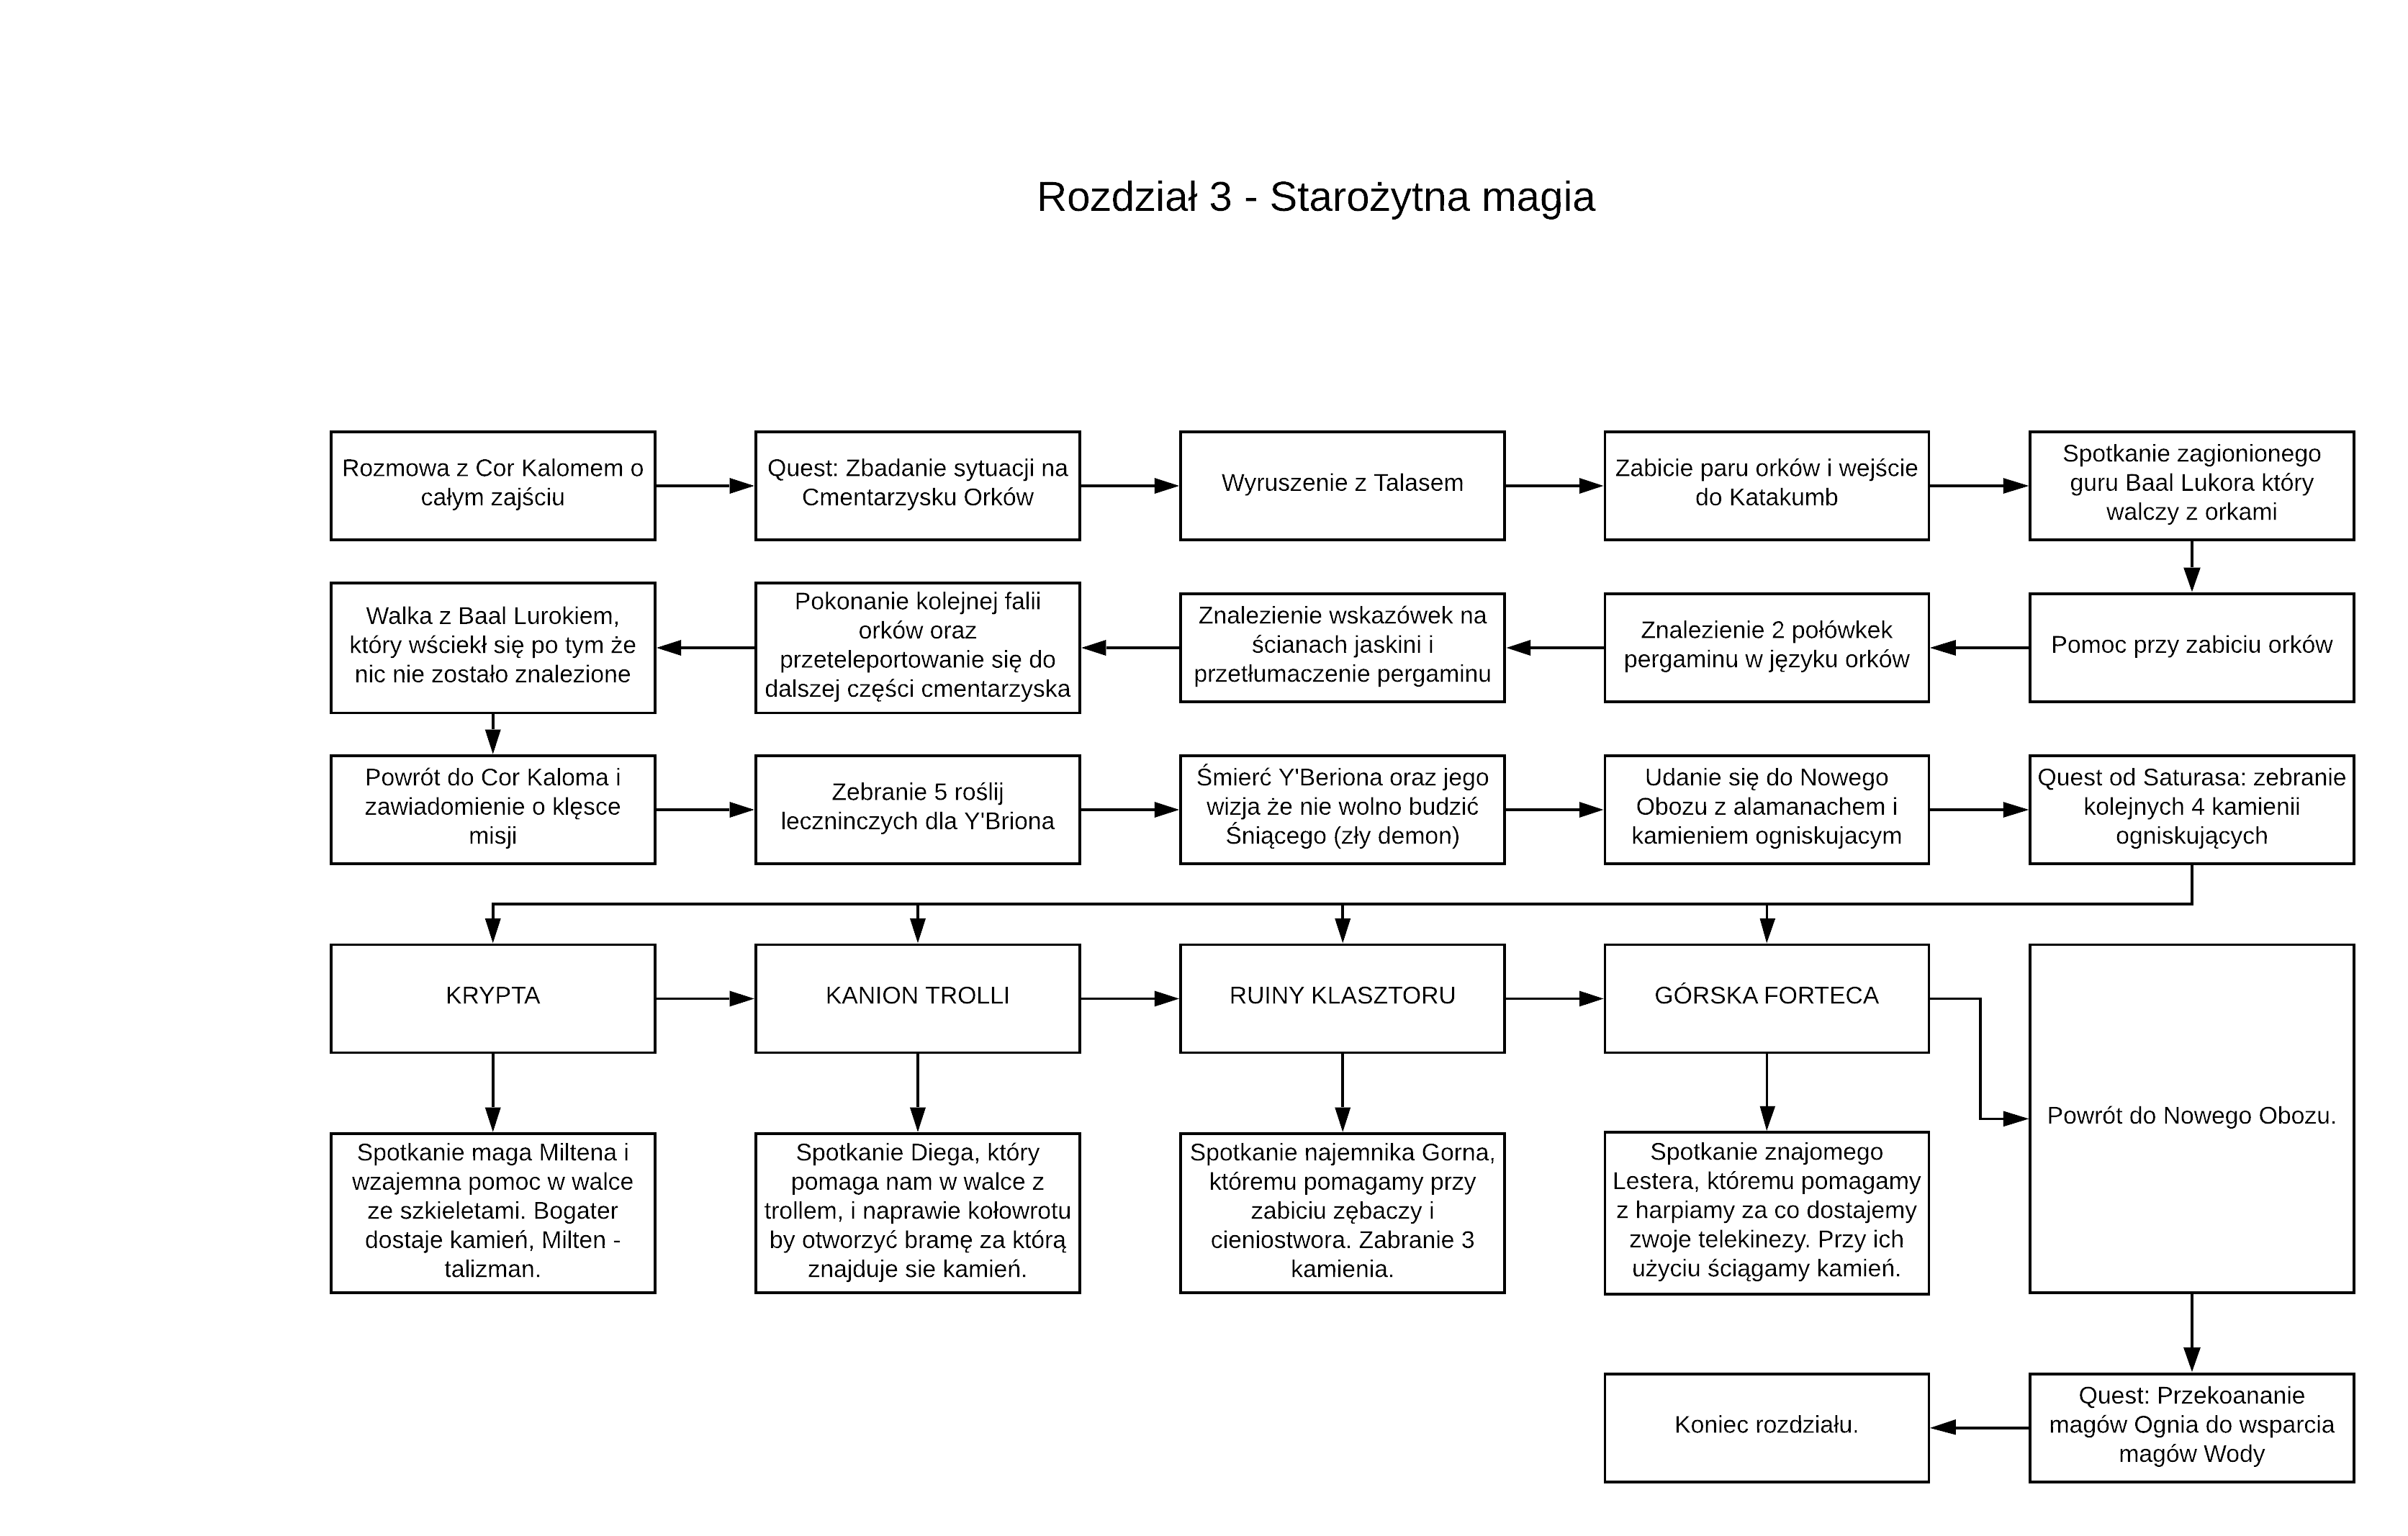
\includegraphics[scale=0.16, angle=90]{rozdzial3}
\end{center}
\section{Rozdział 4 - Xardas}
\begin{center}
	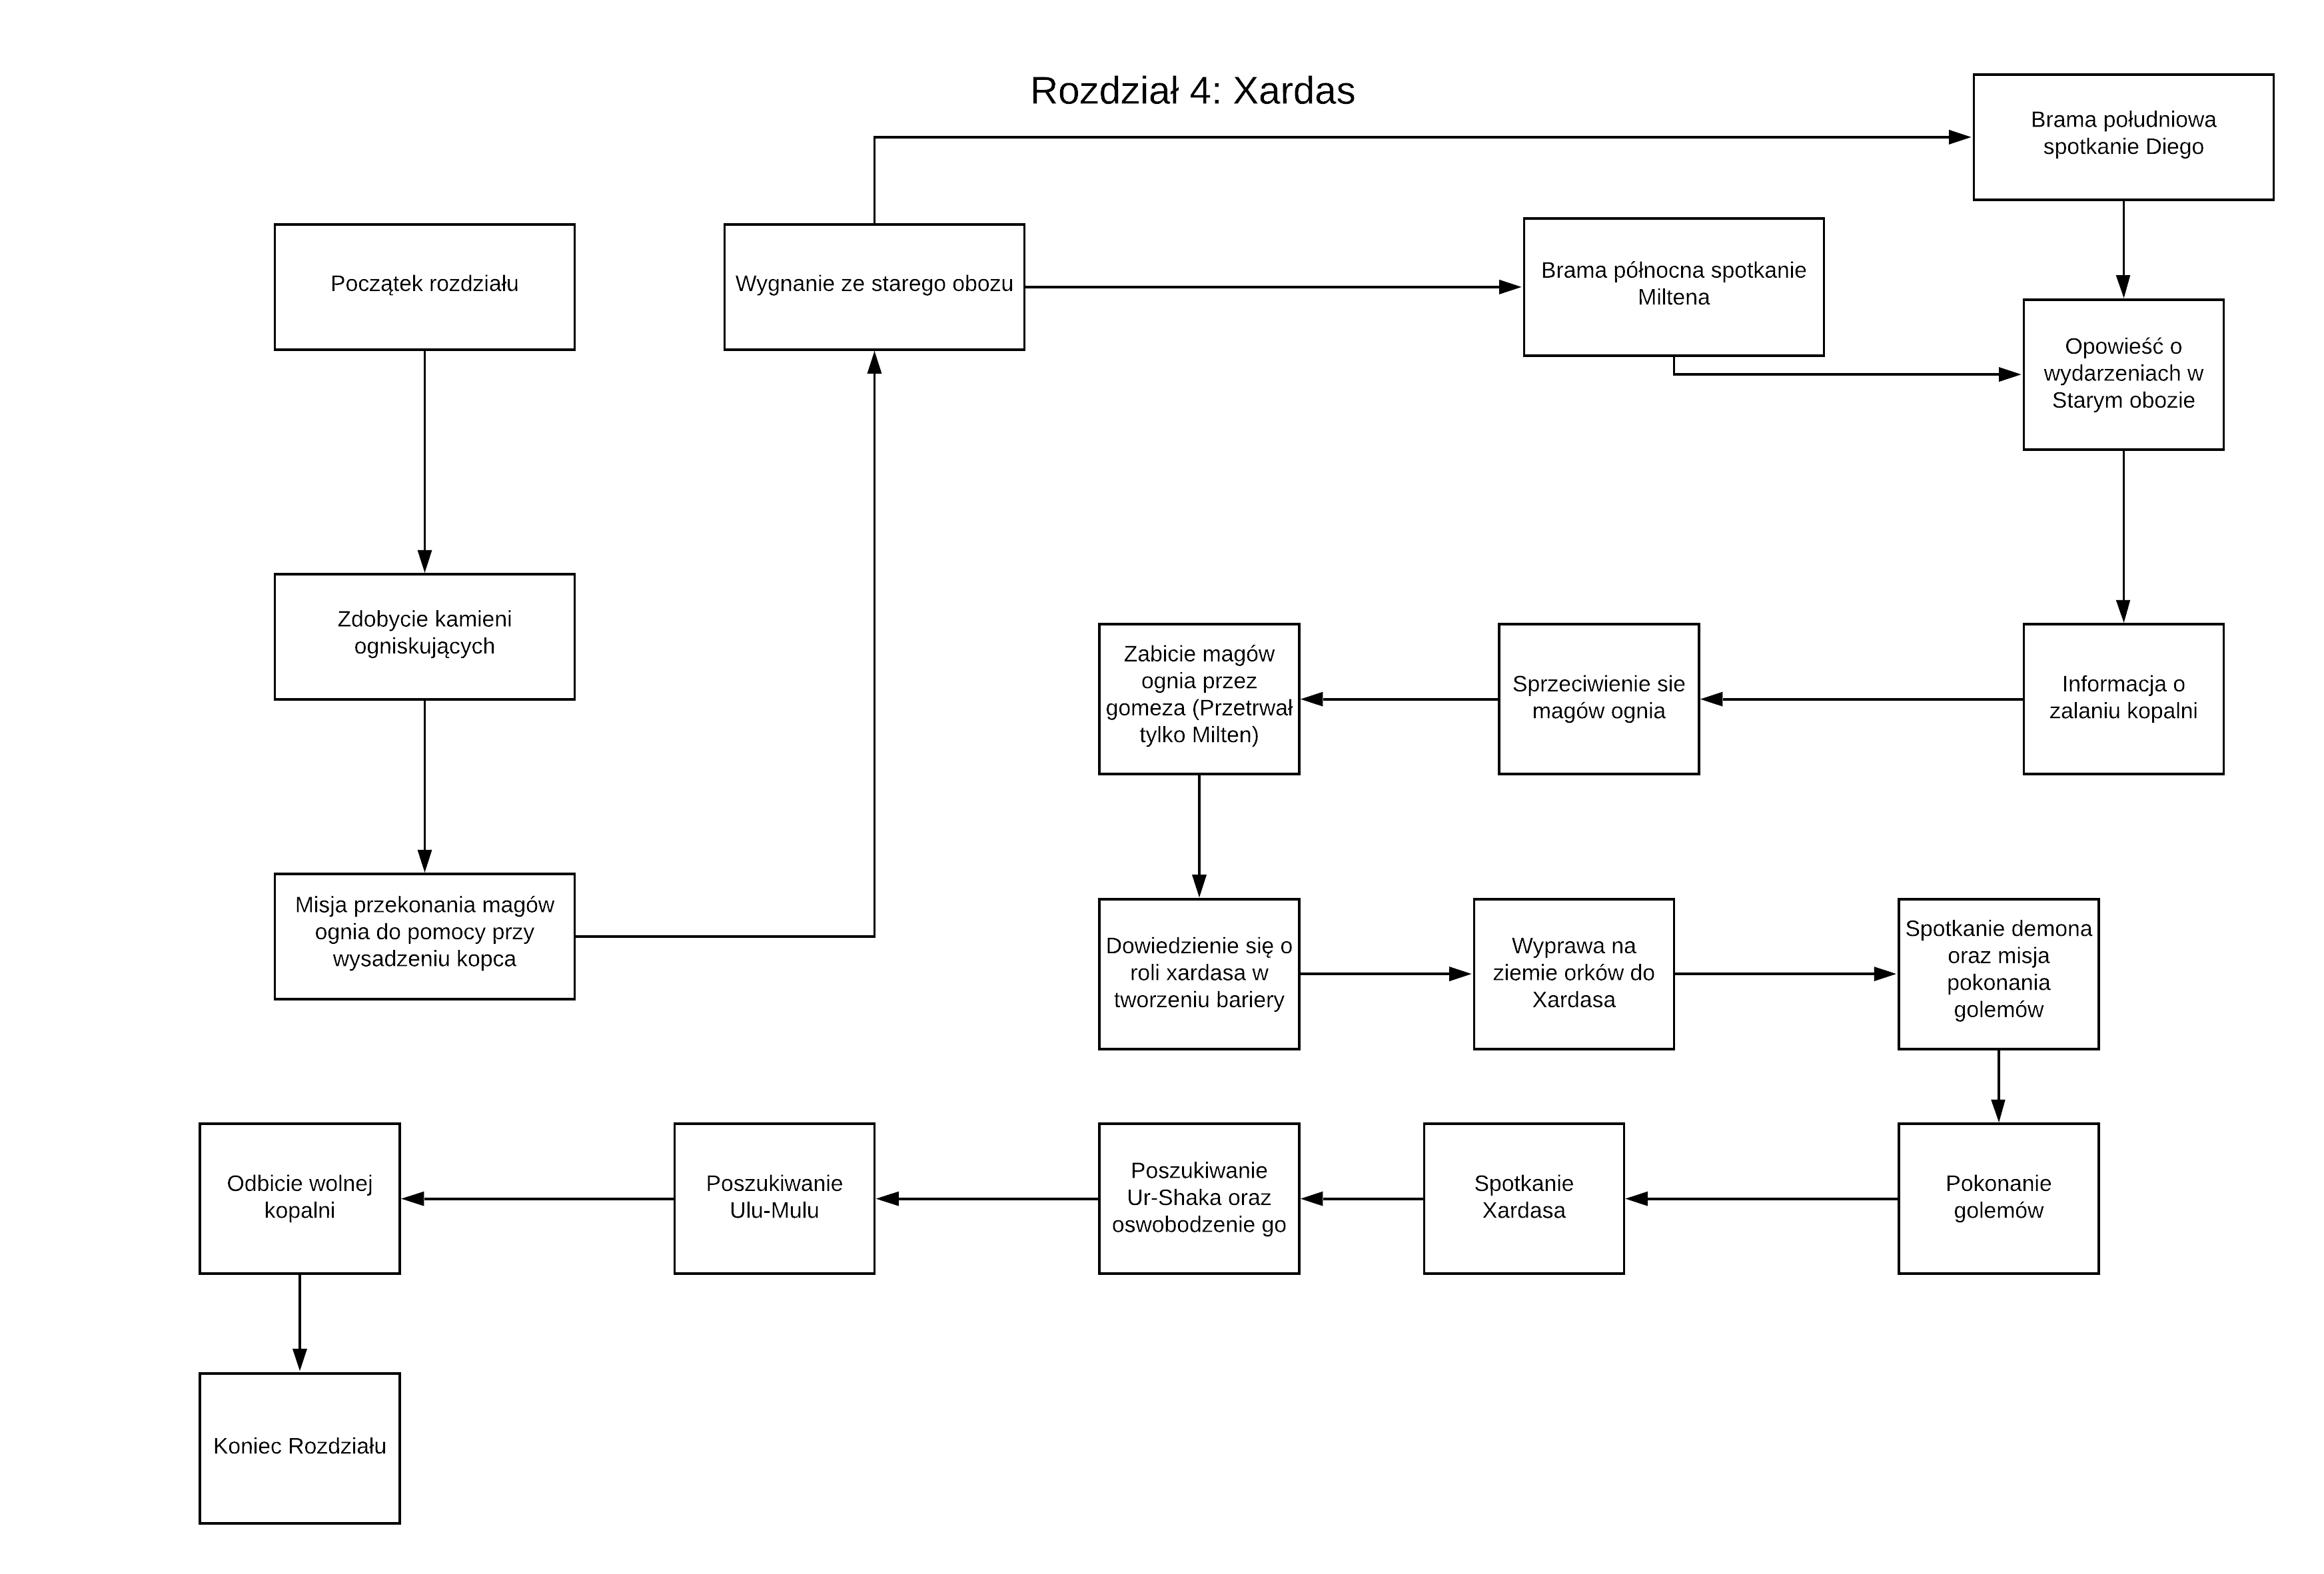
\includegraphics[scale=0.16, angle=90]{4}
\end{center}
\section{Rozdział 5 - Strażnicy portalu}
\begin{center}
	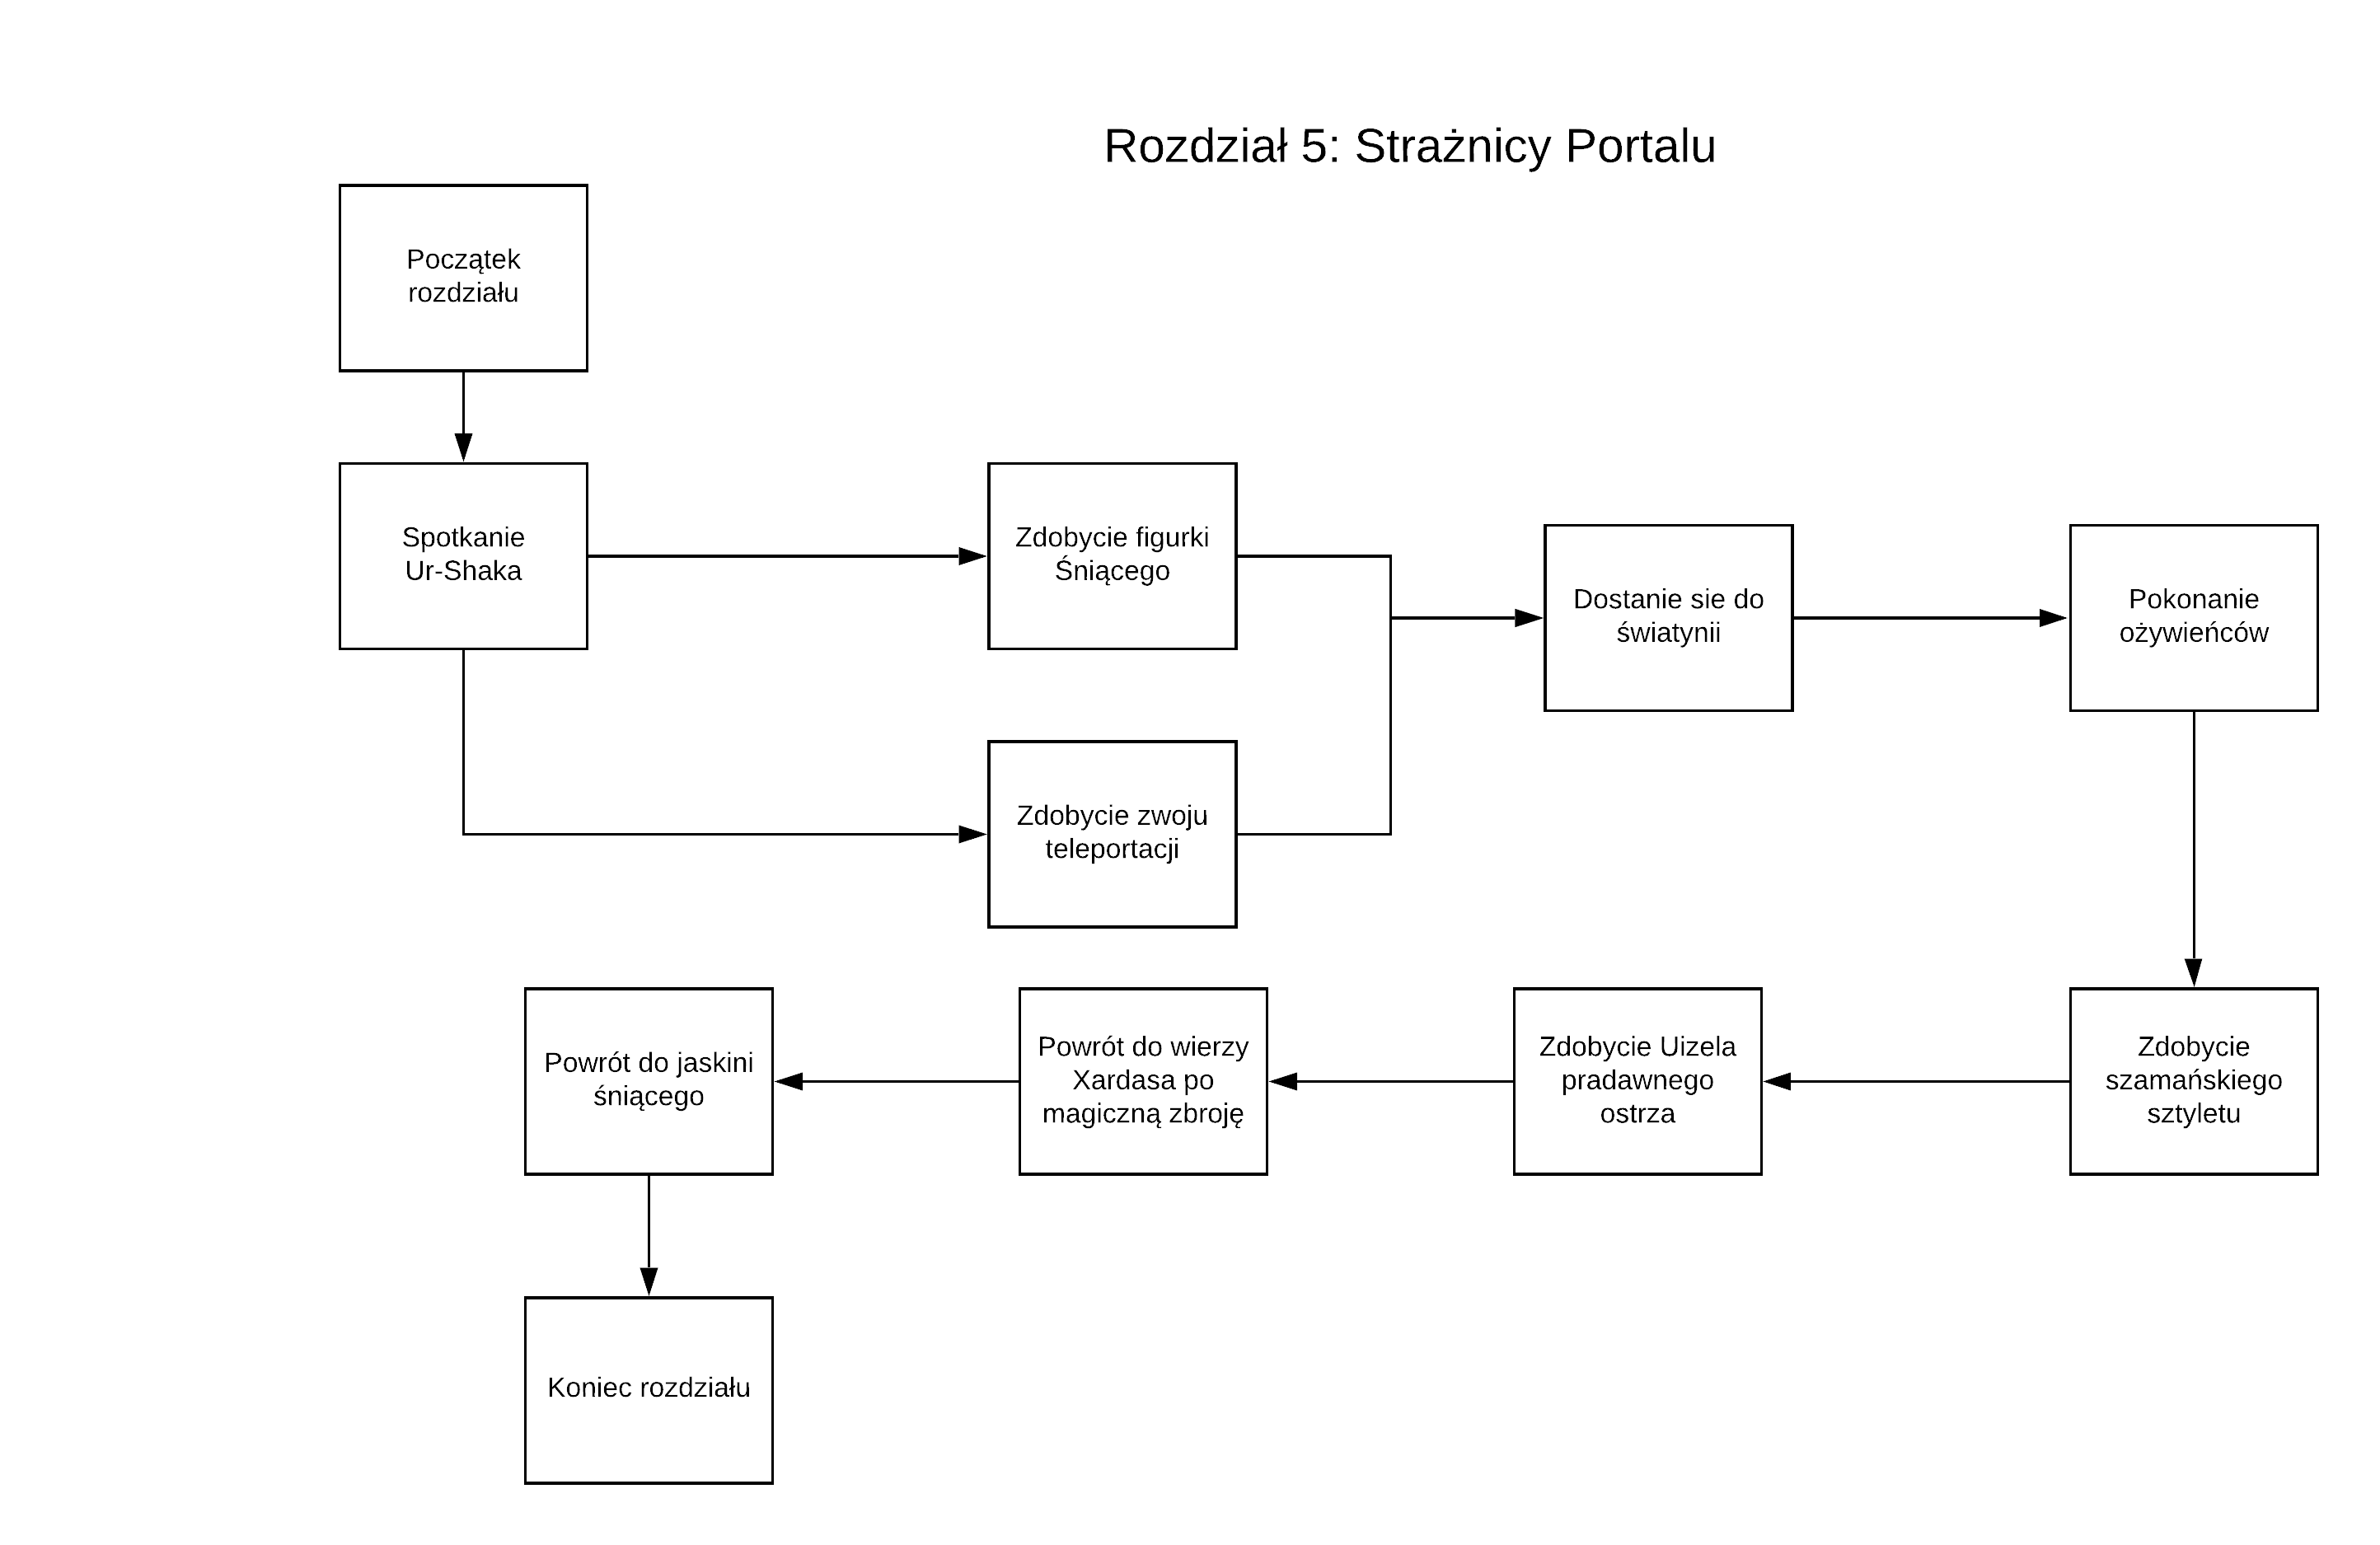
\includegraphics[scale=0.16, angle=90]{5}
\end{center}
\section{Rozdział 6 - Leże śniącego}
\begin{center}
	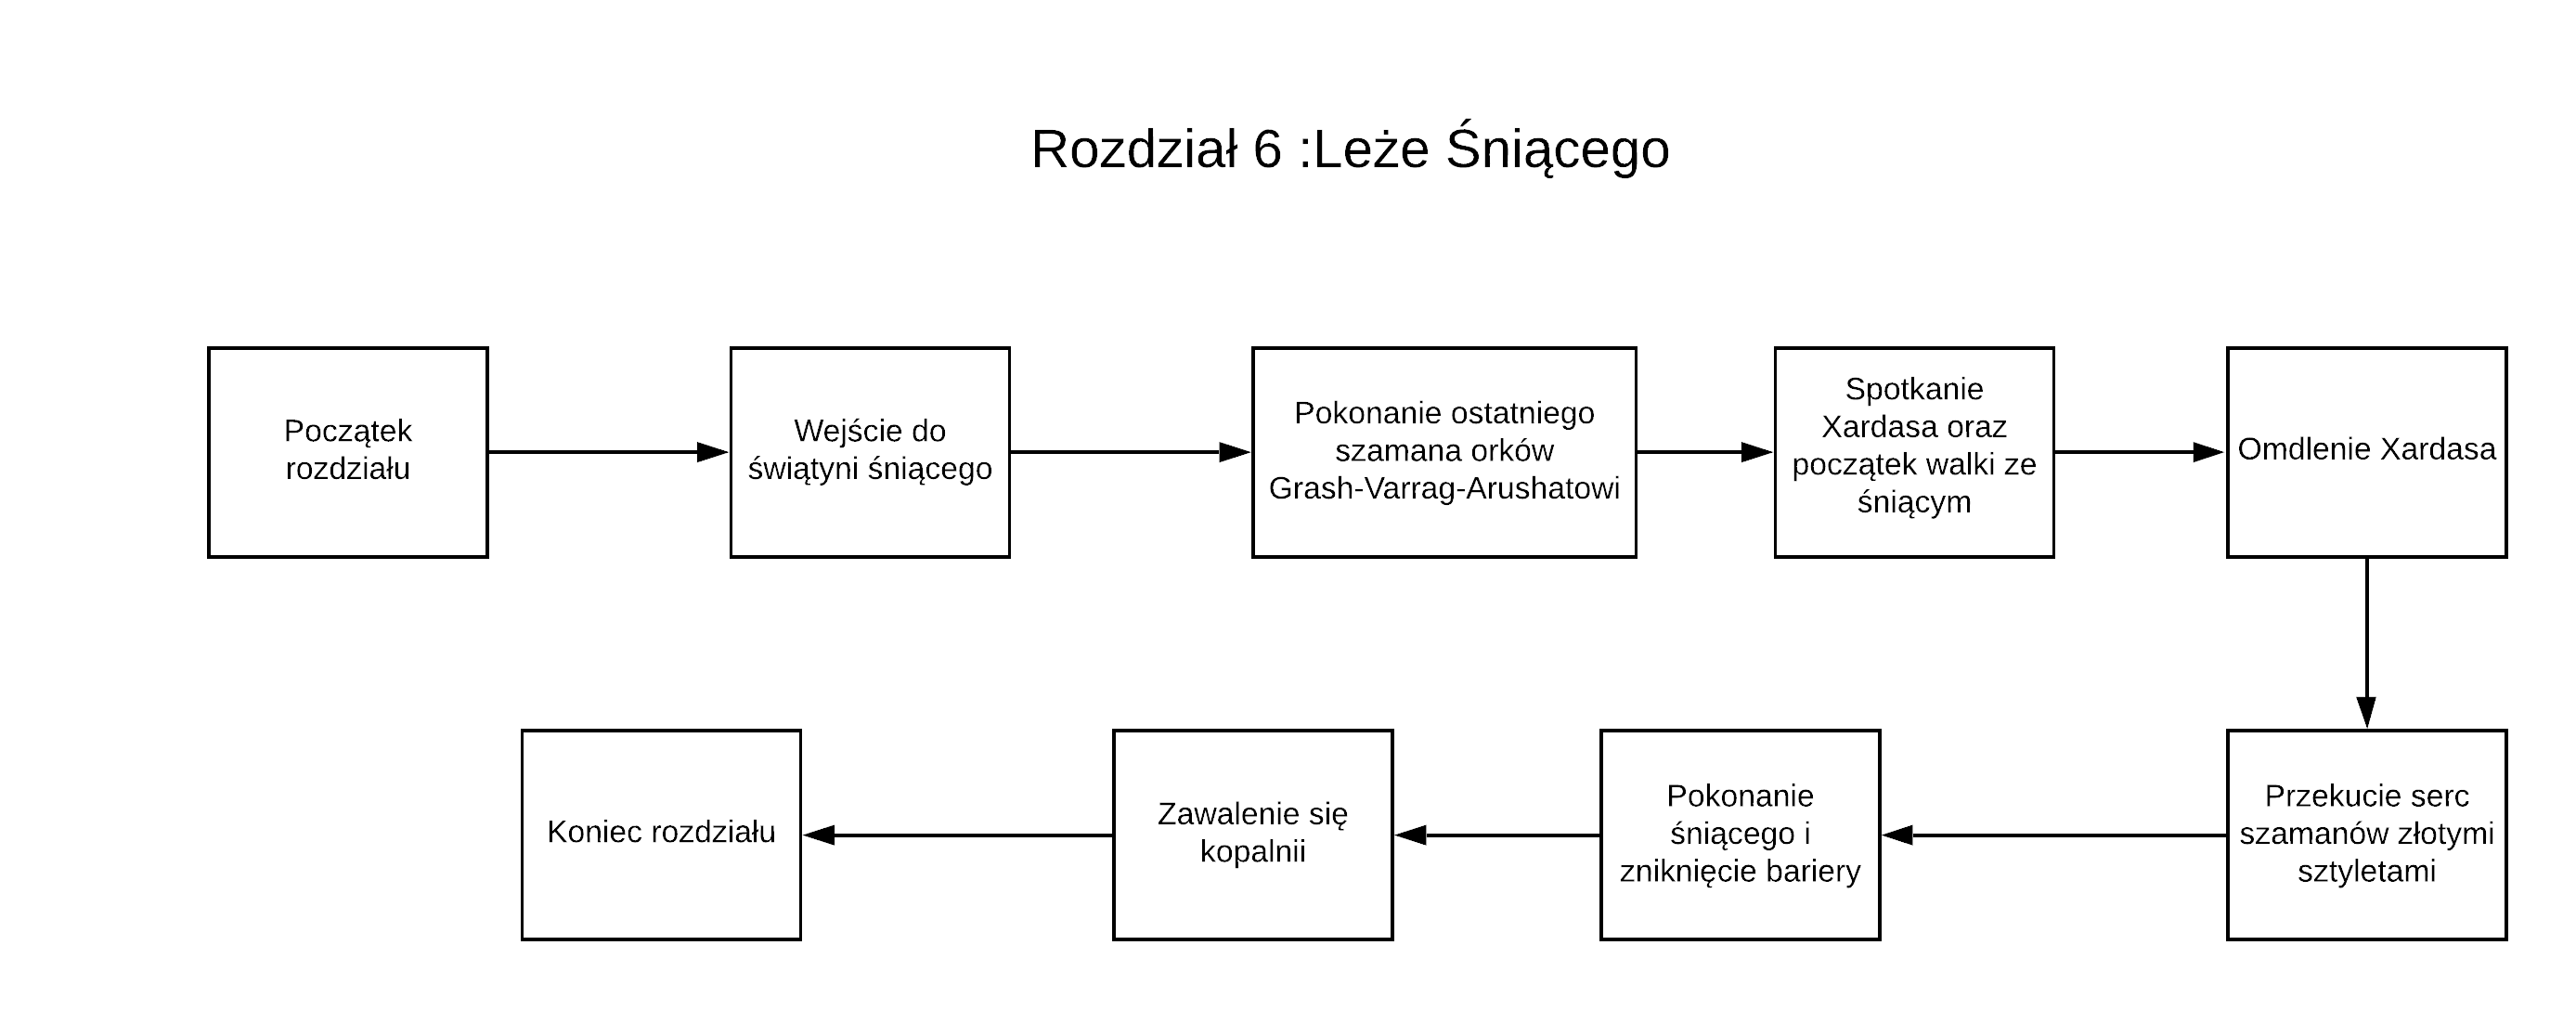
\includegraphics[scale=0.16, angle=90]{6}
\end{center}
\chapter{Rozwój fabuły i zmiany poziomów}\label{chapt:results}
\section{Wstęp}
Gra Gothic jak zostało wyżej wspomniane oferuje w pierwszej części sagi sześć poziomów, które dzielą fabułę na poszczególne sekcje. Gracz wykonując owe postępy na przestrzeni gry poprzez wykonywanie odpowiednich zadań zleconych przez postacie NPC zdobywa punkty doświadczenia, oraz tzw. skille (umiejętności), bez których nie poradziłby sobie w końcowych etapach gry. Pozostając przy etapach stosowanym jest wspomnienie, iż każdy z nich oferuje wiele nagród z wykonane questy, jak również kary za opuszczenie zadania. Poniżej znajduje się opis każdego z rozdziału, który jest swoistym rozwinięciem wyżej wspomnianego flowboarda, który jest pomocny do utworzenia płynnej ścieży fabuły w grze.
\section{Witamy w Kolonii!}
Bezimienny zostaje wrzucony za magiczną barierę, otaczającą Górniczą Dolinę. Głównym zadaniem bohatera w tym rozdziale jest zapoznanie ze światem przedstawionym, mechaniką gry, głównym zaczepieniem fabuły oraz przyłączeniem do któregoś z trzech obozów.
\section{Gniazdo pełzaczy}
Obóz Bractwa przygotowuje się do przyzwania Śniącego. Bohater musi zdobyć na tę okoliczność jeden z pięciu kamieni ogniskujących, jaja królowej pełzaczy i almanach. Następuje wielkie przyzwanie, podczas którego Y'Berion otrzymuje wizję – Śniący kazał im zbadać cmentarzysko orków.
\section{Starożytna magia}
Badanie cmentarzyska orków nie dało żadnych rezultatów. Y'Berion umiera, ostrzegając, że Śniący nie jest tym, za kogo się podawał poprzez wizje i nie należy go budzić. Nadzieja zostaje położona w kopcu rudy magów wody. Bezimienny zbiera w tym celu pozostałe cztery kamienie ogniskujące, po czym staje przed zadaniem przekonania magów ognia, by ci pomogli w detonacji kopca.
\section{Xardas}
Stara Kopalnia uległa zawaleniu, Wolna Kopalnia została zaatakowana przez ludzi Gomeza, a magowie ognia – zamordowani. Magowie wody w desperacji zlecają Bezimiennemu odszukanie dwunastego maga, który brał udział w tworzeniu magicznej bariery – na imię mu było Xardas. Okazuje się, że aby zniszczyć barierę, należy pokonać Śniącego zaszytego głęboko pod ziemią orków.
\section{Strażnicy portalu}
Bohater udaje się w głąb świątyni Śniącego, gdzie pokonuje czterech z pięciu szamanów, którzy brali udział podczas przyzwania wielkiego demona na ten świat. Zdobywa Uriziel – prastary miecz o potężnej sile i mocy. Dzięki pomocy Xardasa udaje się mu przywrócić moc. Początkowo rozdział miał mieć nazwę „Inwazja orków” i miał dotyczyć ataku orków na całą Górniczą Dolinę.
\section{Leże Śniącego}
Bezimienny pokonuje ostatniego z szamanów, by w końcu stawić czoła Śniącemu. Przebija wszystkie pięć szamańskich serc ich własnymi sztyletami, po czym Śniący zostaje wygnany z powrotem do królestwa Beliara, a magiczna bariera upada.
\section{Odbiór gry}
Każdy rozdział gry zostaje rozpoczęty, oraz zakończony krótkim przerywnikiem filmowym, cut scenką prezentującą efekty na który gracz miał bezpośrednio wpływ. Zatem ma on swoisty wpływ jak owy przerywnik będzie wyglądał oraz to co po nim nastąpi. Niektóre postacie NPC mogą zatem zacząć być wrogo nastawione do naszego protagonisty, niektóre wręcz na odwrót mogą zacząć do niego pałać radością.
\chapter{Scenariusz}\label{chapt:results}
\section{Rozgrywka}
Gra powinna zostać zaprojektowana w taki sposób, by każda osoba posiadająca średniej klasy komputer PC była w stanie cieszyć się płynną rozgrywką. Gracz porusza się po świecie z perspektywy trzeciej osoby. Świat gry jest otwarty. Obszar jest ograniczony uzasadnioną fabularnie magiczną barierą, która zadaje graczowi obrażenia podczas próby przejścia przez nią.
\section{Rozwój postaci}
Zdolności bohatera są opisane za pomocą czterech współczynników: siły, zręczności, many i punktów życia. Postać bohatera może być rozwijana poprzez zdobywanie punktów doświadczenia, co skutkuje zwiększaniem poziomu doświadczenia. Za każdy poziom Bezimienny uzyskuje 10 punktów umiejętności oraz zwiększa się ilość jego punktów życia. Punkty umiejętności można spożytkować na naukę wybranej przez siebie umiejętności, bądź na podniesienie poziomu współczynników. W tym celu należy odnaleźć bohatera niezależnego pełniącego rolę nauczyciela. Poza niezależnymi nauczycielami niektórzy bohaterowie niezależni zgodzą się szkolić postać gracza pod warunkiem przynależności do określonej frakcji. Współczynniki można też zwiększyć spożywając niektóre eliksiry i pokarmy. Gracz może zdobyć takie umiejętności jak: posługiwanie się bronią jednoręczną, dwuręczną, łukami, kuszami, otwieranie zamków wytrychem, skradanie się, akrobatykę, kradzież kieszonkową oraz oprawianie zwierząt. Kolejne kręgi magii, umożliwiające dostęp do silniejszych zaklęć, bohater może opanowywać na tej samej zasadzie, co umiejętności.
\section{Frakcje}
W początkowym etapie gry bohater musi zostać członkiem jednej z dostępnych frakcji, aby przejść do dalszego ciągu rozgrywki. Postać gracza może zostać członkiem jednego z trzech obozów. W każdym z nich przynależy do jednego z dostępnych w danym obozie stanowisk, zwanych w grze gildiami. Awans bohatera na poszczególne gildie jest hierarchiczny i w większości przypadków liniowy, a rezygnacja ze stanowiska nie jest możliwa. W zależności od obozu nazwy dostępnych gildii to: cień, a następnie strażnik lub mag ognia – w Starym Obozie; W Nowym Obozie kolejno: szkodnik, najemnik, mag wody; W Bractwie Śniącego: nowicjusz i strażnik świątynny. Wybór gildii ma wpływ na dostęp do nauczycieli, u których można podwyższać statystyki postaci, oraz decyduje o dostępnym graczowi opancerzeniu. Przynależność nie ma znaczącego wpływu na przebieg fabuły. Wybór gracza teoretycznie nie ma także wpływu na możliwą ścieżkę rozwoju postaci – jako członek każdego z obozów bohater ma dostęp do nauczycieli wszystkich rodzajów umiejętności – włączywszy w to nauczycieli niezależnych. Tym niemniej w przypadku Bractwa Śniącego możliwości rozwoju postaci maga są ograniczone.
\section{Sterowanie}
Sterowanie w Gothic, jest bardzo dobre, posiada niestety jedną wadę - przy pierwszym zetknięciu z grą wymaga krótkich ćwiczeń, a następnie przyzwyczajenia. Poznanie oraz zastosowanie się do wszystkich opcji kontrolowania naszą postacią znacznie ułatwi nam grę.
Do dyspozycji mamy klawiaturę i mysz. Należy uważać ją za dodatek, ponieważ gra pierwotnie miała czerpać jedynie z klawiatury. Na początku sterowanie może wydawać się trochę trudne, jednak gdy gracz się go nauczy, będzie gładko przechodzić przez rozgrywkę.
\subsection{Poruszanie się}
Góra/Dół/Lewo/Prawo
Wykonywać manewry naszą postacią możemy dzięki standardowemu Góra/Dół/Lewo/Prawo, a dodatkowo obracać się o dowolny kąt można myszą. Wszystkie te rzeczy da się skonfigurować w opcjach.
\subsection{Podstawowa kombinacja}
Lewy Control (użyj) + Góra
Najczęściej używaną kombinacją jest właśnie ta. Służy do wykonywania większości czynności w grze. Posługując się tym zestawem można podnosić najróżniejsze przedmioty (przedtem należy nakierować się na nie, by wyświetliła się ich nazwa), służy także do interakcji z otoczeniem (rozpoczęcia rozmowy, wspinania się po drabinie, otwierania skrzyni/drzwi itp.).
\subsection{Aktywowanie broni/Czarów}
Spacja
Używając spacji wyciągamy lub chowamy broń i aktywujemy zaklęcie na runie lub zwoju (spacja wywołuje broń lub czar, którego użyto ostatnim razem). Stosując w ataku magię, jest ona przydatna, np. do wybierania czarów - gdy przytrzymamy spację i zaczniemy naciskać Lewo/Prawo.
\subsection{Rozglądanie się}
Klawisz '0'
Przytrzymując ten klawisz będziesz mógł porozglądać się w widoku pierwszej osoby (FPP). Przydatne w przypadku ciasnych pomieszczeniach lub gdy automatyczna kamera nie chce poprawnie współpracować.
\subsection{Skok w przód i wspinanie się}
Alt (skok) + Góra, Alt (skok) + Dół
Postać skoczy do przodu gdy przytrzymasz lewy Alt i klikniesz klawisz Góra. Posiadając umiejętność akrobatyki skoki będą o wiele dłuższe i bezpieczniejsze. Będąc przemienionym w Krwiopijcę, można wykorzystać pewien błąd w grze... Wspomniana kombinacja służy także do wspinania się na różne półki skalne, przedtem trzeba ustawić się twarzą do ściany. Korzystając z Alt + Dół można zeskoczyć z miejsca, na którym wisimy.
\subsection{Zmiana szybkości chodu}
Shift (chodzenie) + Góra
Sprawia, że biegasz wolniej niż normalnie bez używania tej kombinacji. Przydatne przy wysokich miejscach, gdzie poruszanie jest utrudnione (postac dochodzi do krawędzi miejsca, na którym stoi, ale z niej nie spadnie).
\subsection{Zmiana rodzaju broni}
Spacja + Góra/Dół
Kombinacja zmienia aktywny rodzaj broni, pod koniec wybierając go. Jest przydatna gdy postać posługuje się na zmianę bronią do walki w zwarciu, dalekosiężną i magiczną. Posługując się nią, nie trzeba wybierać rodzaju broni za pomocą klawiszy od 0-9.
\subsection{Skradanie się}
Klawisz 'A'
Jeśli posiadasz umiejętność Skradania się, możesz wykorzystywać klawisz 'A' do przejścia w cichy, złodziejski tryb.
\subsection{Okienko z umiejętności}
Klawisz 'S'
W tym okienku możesz zobaczyć swój aktualny poziom, ilość doświadczenia i wszystkie inne statystyki powiązane z umiejętnościami.
\subsection{Dziennik}
Klawisz 'L'
Za każdym razem, gdy ujrzysz informację o zaktualizowaniu swojego podręcznego dziennika, notatnika, będziesz mógł przeczytać w nim nowe informacje zgromadzone najczęściej podczas rozmowy. Można tutaj sprawdzać także wykonane zadanie i te, które zakończyły się niepowodzeniem, dowiedzieć się o aktualnej godzinie w świecie Gothic itp.
\subsection{Enter}
Służy do potwierdzania w opcjach dialogowych przy rozmowach, handlowaniu. Używając Entera można ponownie przemienić się w człowieka po użyciu czaru przemiany w jakiegoś potwora lub zwierzę.
\subsection{Mysz}
Lewy przycisk myszy
Służy do potwierdzania w opcjach dialogowych przy rozmowach, handlowaniu.
Prawy klawisz myszy
Służy do przerywania aktualnie mówionego dialogu podczas rozmowy.
\subsection{Ekwipunek}
Klawisz 'Tab'
Po wciśnięciu tabulatora pojawi się na ekranie kolumna. Cały ekwipunek jest podzielony na kilka grup: Bronie, Zbroje, Artefakty, Magia (runy i zwoje), Jedzenie i napoje, Eliksiry oraz Różne. W grupie Broni, łuki i kusze są ułożone na dole pod bronią białą. Do poruszania się pomiędzy głównymi kolumnami służą Lewo i Prawo, a podświetlanie przedmiotów przez Góra i Dół (ten sam efekt uzyskujemy dzięki scrollce w myszce).
Wybieranie następuje przez posłużenie się główną kombinacją Lewy Ctrl (użyj) + Góra - jedzenie i pożywienie zostanie zjedzone, pierścienie z amuletami i zbrojami są automatycznie zakładane, a bronie i czary zostaną aktywowane pod wolnymi klawiszami wyboru broni (ostatnio używana będzie widoczne także na plecach lub przy pasie). By np. ściągnąć jakąś rzecz używamy ponownie powyższej kombinacji, natomiast gdy chcemy coś porzucić/upuścić - stosujemy Lewy Ctrl (użyj) + Góra.
Dzięki klawiszom wyboru (1-0) możemy szybko wybrać jakąś broń. Broń biała jest umiejscowiona pod '1', broń dystansowa pod '2', ostatnio używany czar to '3', a od 4 do 0 dostępne są wybrane czary.
\subsection{Opróżnianie z zawartości skrzyń}
Lewy Ctrl (użyj) + ruch w bok
Stań naprzeciw skrzyni, przytrzymaj Lewy Ctrl (użyj) i naciśnij Góra. Po lewej stronie ekranu pojawi się zawartość skrzyni, która nie jest pogrupowana, a po prawej standardowo nasz ekwipunek. Przenieś się do przedmiotów z lewej strony, przytrzymaj Lewy Ctrl (użyj) i naciśnij Prawo (klikając Lewo w naszym ekwipunku przedmiot zostanie włożony do skrzyni).
Jeśli chcesz przenosić więcej niż jedną rzecz, użyj tych kombinacji:
Lewy Ctrl (użyj) + obrót w lewo/prawo - jednorazowo przenosi 1 przedmiot
Lewy Ctrl (użyj) + krok w lew/prawo - jednorazowo przenosi 10 przedmiotów
Lewy Ctrl (użyj) + obrót w lewo/prawo + Shift - jednorazowo przenosi 100 przedmiotów
\subsection{Handlowanie}
Lewy Ctrl (użyj) + ruch w bok
Handlowanie jest bardziej skomplikowane niż opróżnianie skrzyń, ale nie powinno nastręczać problemów. Do ekranu handlowania przechodzi się po wybraniu odpowiedniej opcji dialogowej przy rozmowie z jakimś NPCem. Pojawiają się dwie kolumny po lewej i prawej stronie (tak, jak podczas opróżniania skrzyń) oraz dodatkowo dwie kolumny pośrodku ekranu. Przy przenoszeniu towarów, będą one najpierw umieszczane w środkowych kolumnach, na samej górze wyświetlą się zsumowana wartość wszystkich kupowanych i sprzedawanych przedmiotów. Możesz kupować i oferować tyle towarów, ile chcesz. By transakcja powiodła się, suma wartości sprzedawanych rzeczy musi być większa lub równa od sumy wartości kupowanych rzeczy. Jeśli będzie to się zgadzać, przejdź do którejś z środkowych kolumn i naciśnij Enter, a następnie wybierz opcję "Przyjmij". Przedmioty zostaną automatycznie posegregowane w ekwipunku, więc nie trzeba zawracać sobie głowy ich układaniem. Przy handlowaniu, szczególnie w późniejszych rozdziałach warto stosować bryłki rudy jako nominał. Nie polecam kolekcjonowania mało lub wcale wartościowych rzeczy, ponieważ zaśmiecają ekwipunek, a podczas sprzedawania są mieszane z towarami przyjmującego, wyjątkiem są oczywiście przedmioty potrzebne lub przydatne do wykonywania zadań.
Jeśli chcesz przenosić więcej niż jedną rzecz, użyj tych kombinacji:
Lewy Ctrl (użyj) + obrót w lewo/prawo - jednorazowo przenosi 1 przedmiot
Lewy Ctrl (użyj) + krok w lew/prawo - jednorazowo przenosi 10 przedmiotów
Lewy Ctrl (użyj) + obrót w lewo/prawo + Shift - jednorazowo przenosi 100 przedmiotów
\subsection{Kradzież kieszonkowa}
Lewy Ctrl (użyj) + ruch w bok
Okradanie NPCów wymaga cichego podskradania się do celu, dlatego w odległości kilku metrów od "ofiary" (tak, by nie wyczuwała naszej obecności) należy kliknąć klawisz 'A'. Zachodzimy ją od tyłu, a przy dostatecznie bliskiej odległości postępujemy tak samo, jak w przypadku opróżniania z zawartości skrzyń (opisane wyżej). Nie można przy tym zwrócić niczyjej uwagi, ponieważ NPCe informują się nawzajem o zagrożeniach. Przy niskiej ilości zręczności oraz poziomie umiejętności kradzieży naszej postaci należy zwracać szczególną uwagę i nie zabierać wszystkiego naraz oraz działać szybko, ponieważ nasz cel może szybko zorientować się, że go oszukujemy...
\subsection{Spanie}
Lewy Ctrl (użyj) + Góra
Stań z boku łóżka będąc skierowanym twarzą w jego stronę i zastosuj standardową kombinacją: Lewy Ctrl (użyj) + Góra. Postać położy się na łóżko, a w okienku dialogowym pojawią się opcje długości spania, np. "Śpij do rana". Wybierz jedną z nich, a gdy się obudzisz naciśnij klawisz 'w bok', by wstać z łoża. Możesz spać na każdym posłaniu, przy czym nie musisz ścielić.
\subsection{Pływanie i nurkowanie}
Klawisze poruszania się
Wejdź do wody, przejdź na głębię, ponieważ dopóki twoje nogi będą dotykały dna, będziesz powoli brodził. Pływanie nad wodą odbywa się poprzez używanie klawiszów odpowiedzialnych za poruszanie się postaci (Góra, Dół, Lewo, Prawo).
Aby zanurkować kliknij Prawy Przycisk Myszy lub Alt (klawisz skoku). Tak długo, jak będziesz trzymać przycisk myszy pod wodą, będziesz płynąć przed siebie. Kierunek zmienia się manewrując myszą lub używając klawiszy poruszania się. Jeśli chcesz wypłynąć na powierzchnię, to podpłyń głową do lustra wody i raz kliknij Prawy Przycisk Myszy. Zawsze kontroluj zapas swojego tlenu pod wodą, który wskazuje żółty pasek.
\subsection{Minimalne wymagania sprzętowe}
Pentium II 300Mhz (zalecany Pentium III 800 Mhz)
128 MB pamięci RAM (zalecane 256 MB)
CD-ROM 8x / DVD-ROM
Akcelerator grafiki 3D (zalecane 32 MB RAM)
Karta dźwiękowa zgodna z DirectX
Windows 95/98/Me/2000/XP
\pagebreak


% Adding a bibliography if citations are used in the report
\bibliographystyle{plain}
\bibliography{bibliography.bib}
% Adds reference to the Bibliography in the ToC
\addcontentsline{toc}{chapter}{\bibname}

\pagebreak

\chapter*{Appendix A: Resources}
[\textit{Report the config files of the software used (i.e. SU2 \cite{economon2015su2} and the mesher). Also attach to this report an archive with the mesh files, solutions and the reference solution data (e.g. data points of a Cp plot ...)}]
\section*{Mesh configuration files}
\section*{SU2 configuration files}
% \section{Reference solution data}


\end{document}
